% Set a pdf version and a document type
\ifx\pdfminorversion\undefined\else\pdfminorversion=4\fi
\documentclass[aspectratio=169,t,table]{beamer}

% Import all necessary packages
% Use this file to import all packages which are needed for the lecture
\usepackage[english]{babel}
\usepackage[utf8]{inputenc}
\usepackage[sfdefault]{roboto}
\usepackage[T1]{fontenc}
\usepackage{amsmath,amssymb}
\usepackage{graphicx}
\usepackage{listings}
\usepackage[backend=biber,sorting=none,doi=true,style=ieee]{biblatex}
\usepackage{url}
\usepackage{hyperref}
\usepackage{fontawesome5}
\usepackage{graphicx}
\usepackage{booktabs}
\usepackage{calc}
\usepackage{ifthen}
\usepackage{tabularx}
\usepackage{longtable}
\usepackage{makecell}
\usepackage{multicol}
\usepackage{multirow}
\usepackage{hhline}
\usepackage{qrcode}
\usepackage{xcolor}
\usepackage{cleveref}
\usepackage{tikz}
\usepackage{tikz-cd}
\usepackage{pgfplots,pgfplotstable,pgf-pie}
\usepackage[linesnumbered]{algorithm2e}
\usepackage{array}
\usepackage{mathtools}
\usepackage{verbatim}
\usetikzlibrary{patterns}
\usetikzlibrary{arrows.meta}


% Set the theme (customized FAU beamer theme)
\usetheme[%
	image,%
	longtitle,%
	inst=tf%
]{fau}

% Set all important settings and define commands that are used in more than one lecture
% Set institute and date 
\institute[CS6]{Computer Science 6 (Data Management), Friedrich-Alexander-Universit\"at Erlangen-N\"urnberg}
\date[SS\the\year{}]{Summer semester \the\year{}}

% Configure the bibliography
\defbibheading{bibliography}{}
\addbibresource{references.bib}

% Define additional colors 
\definecolor{airforceblue}{rgb}{0.36, 0.54, 0.66}
\definecolor{ForestGreen}{rgb}{0.34, 0.139, 0.34}

% Configure the template
\setbeamercovered{transparent}
\setbeamertemplate{section in toc}[sections numbered]
\setbeamertemplate{section page}{%
	\begingroup
	\begin{beamercolorbox}[sep=10pt,center,rounded=true,shadow=true]{section title}
		\usebeamerfont{section title}\thesection~\insertsection\par
	\end{beamercolorbox}
	\endgroup
}
\setlength{\skip\footins}{0.2cm}
\setlength{\footnotesep}{0.1cm}

% Configure the formatting of listings
\lstset{%
	language=Python,
	tabsize=2,
	basicstyle=\tt,
	keywordstyle=\color{blue},
	commentstyle=\color{green!50!black},
	stringstyle=\color{red},
	numbers=left,
	numbersep=0.5em,
	xleftmargin=1em,
	numberstyle=\tt
}

% Add tikz and pgfplots libraries
\usetikzlibrary{arrows,decorations.pathmorphing,backgrounds,fit,positioning,shapes.symbols,chains,intersections,snakes,positioning,matrix,mindmap,shapes.multipart,shapes,calc,shapes.geometric,shadows,shadows.blur}
\usepgfplotslibrary{groupplots}

% Define pgfplotsset
\pgfplotsset{height=4cm,width=8cm,compat=1.14}

% Define tikz sets 
\tikzset{
	every overlay node/.style={
			anchor=north west, inner sep=0pt,
		},
}
\tikzset{
	thick,
	>=latex,
	every edge/.style={draw=gray, thick, >=latex},
	vertex/.style = {
			circle,
			fill            = black,
			outer sep = 2pt,
			inner sep = 1pt,
		}
}
\tikzset{level 1/.append style={sibling angle=50,level distance = 165mm}}
\tikzset{level 2/.append style={sibling angle=20,level distance = 45mm}}
\tikzset{every node/.append style={scale=1}}
\tikzset{
	vertex/.style = {
			circle,
			fill            = black,
			outer sep = 2pt,
			inner sep = 1pt,
		}
}
\tikzset{
	mynode/.style={
			draw,
			thick,
			anchor=south west,
			minimum width=2cm,
			minimum height=1.3cm,
			align=center,
			inner sep=0.2cm,
			outer sep=0,
			rectangle split,
			rectangle split parts=2,
			rectangle split draw splits=false},
	reverseclip/.style={
			insert path={(current page.north east) --
					(current page.south east) --
					(current page.south west) --
					(current page.north west) --
					(current page.north east)}
		}
}
\tikzset{basic/.style={
			draw,
			rectangle split,
			rectangle split parts=2,
			rectangle split part fill={blue!20,white},
			minimum width=2.5cm,
			text width=2cm,
			align=left,
			font=\itshape
		},
	Diamond/.style={ diamond,
			draw,
			shape aspect=2,
			inner sep = 2pt,
			text centered,
			fill=blue!10!white,
			font=\itshape
		}
}

% Define tikzoverlay
% Usage:
% \tikzoverlay at (-1cm,-5cm) {content};
% or
% \tikzoverlay[text width=5cm] at (-1cm,-5cm) {content};
\def\tikzoverlay{%
	\tikz[remember picture, overlay]\node[every overlay node]
}%

% Define additional math operators
\DeclareMathOperator*{\argmax}{arg\,max}
\DeclareMathOperator*{\argmin}{arg\,min}

% Define pgfmath functions
\pgfmathdeclarefunction{gauss}{2}{%
	\pgfmathparse{1/(#2*sqrt(2*pi))*exp(-((x-#1)^2)/(2*#2^2))}%
}

% Define additional commands
\newcommand*{\fullref}[1]{\underline{\hyperref[{#1}]{\cref{#1} (\nameref*{#1})}}}
\newcommand{\tikzmark}[1]{\tikz[remember picture] \node[coordinate] (#1) {#1};}
\newcommand{\plots}{0.611201}
\newcommand{\plotm}{2.19882}
\newcommand{\MaxNumberX}{3}
\newcommand{\MaxNumberY}{5}


% Title, author(s), and date
\title[KDD~7.~Classification]{7. Classification} %
\subtitle{Knowledge Discovery in Databases}
\author[D.~Probst]{Dominik Probst, \texttt{Dominik.probst@fau.de}}
\input{x-additional/vc.tex}

\hypersetup{
	pdfkeywords={},
	pdfsubject={Version \GITAbrHash},
	pdfcreator={},
	pdflang={English}
}


% Create custom commands
\newcommand\mycommfont[1]{\footnotesize\ttfamily\textcolor{faucyan}{#1}}
\newcommand*\revealcline{\noalign{\vskip\arrayrulewidth}} % used in 5-evaluation-selection

% Set custom (theme) settings 
\setbeamercovered{invisible}
\SetCommentSty{mycommfont}

% Start the document
\begin{document}

% Title
\maketitle

{ % Outline
	\setbeamertemplate{footline}{}
	\begin{frame}[noframenumbering]{Outline}
		\tableofcontents

	\end{frame}
}

% Body
\section{Basic Concepts}

\begin{frame}{Supervised vs. Unsupervised Learning}
	\begin{columns}
		\begin{column}{0.5\textwidth}
			\textbf{Supervised Learning}
			\begin{itemize}
				\item The \textbf{training data} (observations, measurements, etc.) are accompanied by \textbf{labels} indicating the \textbf{class} of the observations.
				\item New data is classified based on a \textbf{model} created from the training data.
			\end{itemize}

		\end{column}

		\begin{column}{0.5\textwidth}
			\textbf{Unsupervised Learning}

			\begin{itemize}
				\item Class labels of training data are unknown.

				      Or rather, there are no training data.
			\end{itemize}
			\begin{itemize}
				\item Given a set of measurements, observations, etc., the goal is to find classes or clusters in the data.

				      $\rightarrow$ See next chapter (Lecture/Chapter 8: Clustering).
			\end{itemize}

		\end{column}
	\end{columns}
\end{frame}

\begin{frame}{Prediction Problems: Classification vs. Numerical Prediction}
	\begin{itemize}
		\item \textbf{Classification:}
		      \begin{itemize}
			      \item Predicts \textbf{\color{airforceblue}categorical class labels} (discrete, nominal).
			      \item Constructs a model based on the training set and the values (class labels) in a classifying attribute and uses it in classifying new data.
		      \end{itemize}
		\item \textbf{Numerical prediction:}
		      \begin{itemize}
			      \item Models \textbf{\color{airforceblue}continuous-valued functions}.
			      \item I.e. predicts missing or unknown (future) values.
		      \end{itemize}
		\item \textbf{Typical applications of classification:}
		      \begin{itemize}
			      \item Credit/loan approval: Will it be paid back?
			      \item Medical diagnosis: Is a tumor cancerous or benign?
			      \item Fraud detection: Is a transaction fraudulent or not?
			      \item Web-page categorization: Which category is it such as to categorize it by topic.
		      \end{itemize}
	\end{itemize}
\end{frame}

\begin{frame}{Classification -- A Two-step Process}
	\begin{enumerate}
		\item \textbf{Model construction: describing a set of predetermined classes:}
		      \begin{itemize}
			      \item Each tuple/sample is assumed to belong to a predefined class, as determined by the \textbf{\color{airforceblue}class-label attribute}.
			      \item The set of tuples used for model construction is the \textbf{\color{airforceblue}training set}.
			      \item The \textbf{\color{airforceblue}model} is represented as classification rules, decision trees, or mathematical formulae.
		      \end{itemize}
		\item \textbf{Model usage, for classifying future or unknown objects:}
		      \begin{itemize}
			      \item Estimate \textbf{\color{airforceblue}accuracy} of the model:
			            \begin{itemize}
				            \item The known label of \textbf{test samples} is compared with the result from the model.
				            \item \textbf{Accuracy rate} is the percentage of test-set samples that are correctly classified by the model.
				            \item Test set is independent of training set (otherwise overfitting).
				            \item More on evaluation metrics later in \hyperlink{section:evaluation}{\beamergotobutton{section ``Model Evaluation and Selection''}}.
			            \end{itemize}
			      \item If the accuracy is acceptable, \textbf{\color{airforceblue}use the model} to classify data tuples whose class labels are not known.
		      \end{itemize}
	\end{enumerate}
\end{frame}

\begin{frame}{Classification -- A Two-step Process: 1. Model Construction}
	\centering
	\begin{tikzpicture}[
			>=latex,
			database/.style={
					cylinder,
					cylinder uses custom fill,
					cylinder body fill=faublue!12,
					cylinder end fill=faublue!12,
					shape border rotate=90,
					aspect=0.25,
					draw
				}
		]
		\node[database] (data) at (0,0) {Training data};
		\node[below=2em of data] (data-example) {
			\begin{tabular}{|l|l|c|c|}
				\hline
				\cellcolor{faugray!62}\textbf{\uppercase{name}} & \cellcolor{faugray!62}\textbf{\uppercase{rank}} & \cellcolor{faugray!62}\textbf{\uppercase{years}} & \cellcolor{fauorange!25}\textbf{\uppercase{tenured}} \\\hline
				\cellcolor{fauyellow!25}Mike                    & \cellcolor{fauyellow!25}Assistant Prof          & \cellcolor{fauyellow!25}3                        & {\color{faured}no}                                   \\\hline
				\cellcolor{fauyellow!25}Mary                    & \cellcolor{fauyellow!25}Assistant Prof          & \cellcolor{fauyellow!25}7                        & {\color{faugreen}yes}                                \\\hline
				\cellcolor{fauyellow!25}Bill                    & \cellcolor{fauyellow!25}Professor               & \cellcolor{fauyellow!25}2                        & {\color{faugreen}yes}                                \\\hline
				\cellcolor{fauyellow!25}Jim                     & \cellcolor{fauyellow!25}Associate Prof          & \cellcolor{fauyellow!25}7                        & {\color{faugreen}yes}                                \\\hline
				\cellcolor{fauyellow!25}Dave                    & \cellcolor{fauyellow!25}Assistant Prof          & \cellcolor{fauyellow!25}6                        & {\color{faured}no}                                   \\\hline
				\cellcolor{fauyellow!25}Anne                    & \cellcolor{fauyellow!25}Associate Prof          & \cellcolor{fauyellow!25}3                        & {\color{faured}no}                                   \\\hline
			\end{tabular}
		};
		\node[rounded corners=5pt,draw=fauorange,fill=fauorange!62, text width = 3cm, align=center,right=15em of data.east] (class-algo) {Classification\\algorithm};
		\node[database,below=3em of class-algo] (class-rules) {Classification rules};
		\node[draw=faucyan,fill=faucyan!25,text=black,rounded corners=5pt,text width=3cm,below=2em of class-rules] (rules) {\texttt{if RANK =}'Professor'\\\texttt{or YEARS >}6\\\texttt{then TENURED =}'yes'};

		\draw[->,thick] (data) -- (class-algo);
		\draw[->,thick] (class-algo) -- (class-rules);

		\draw[thick,rounded corners=5pt]
		(data-example.north west) -- ($(data-example.north west) + (0,.15)$) --
		($(data-example.north) + (0,.15)$) -- ($(data-example.north) + (0,.15)$) --
		($(data-example.north east) + (0,.15)$) -- (data-example.north east);

		\draw[thick,rounded corners=5pt]
		($(rules.north west) + (-.1,.05)$) -- ($(rules.north west) + (-.1,.25)$) --
		($(rules.north) + (0,.25)$) -- ($(rules.north) + (0,.25)$) --
		($(rules.north east) + (.1,.25)$) -- ($(rules.north east) + (.1,.05)$);
	\end{tikzpicture}
\end{frame}

\begin{frame}{Classification -- A Two-step Process: 2. Model Usage}
	\centering
	\begin{tikzpicture}[
			>=latex,
			database/.style={
					cylinder,
					cylinder uses custom fill,
					cylinder body fill=faublue!12,
					cylinder end fill=faublue!12,
					shape border rotate=90,
					aspect=0.25,
					draw
				}
		]
		\node[database] (data) at (0,0) {Testing data};
		\node[below=2em of data] (data-example) {
			\begin{tabular}{|l|l|c|c|}
				\hline
				\cellcolor{faugray!62}\textbf{\uppercase{name}} & \cellcolor{faugray!62}\textbf{\uppercase{rank}} & \cellcolor{faugray!62}\textbf{\uppercase{years}} & \cellcolor{fauorange!25}\textbf{\uppercase{tenured}} \\\hline
				Tom                                             & Assistant Prof                                  & 2                                                & {\color{faured}no}                                   \\\hline
				\cellcolor{fauyellow!25}Merlisa                 & \cellcolor{fauyellow!25}Associate               &
				\cellcolor{fauyellow!25}7                       & \cellcolor{fauyellow!25}{\color{faured}no}
				\\\hline
				George                                          & Professor                                       & 5                                                & {\color{faugreen}yes}                                \\\hline
				Joseph                                          & Assistant Prof                                  & 7                                                & {\color{faugreen}yes}                                \\\hline
			\end{tabular}
		};
		\node[draw=faucyan,fill=faucyan!25,rounded corners=5pt,text width = 3cm, align=center,right=15em of data.east] (class-algo) {Classification\\rules};
		\node[database,below=3em of class-algo] (new-data) {Unseen data};
		\node[rounded corners=5pt,fill=faugray!12,text width=3.5cm,below=2em of new-data,align=center] (new-data-example) {\texttt{(Jeff, Professor, 4)}};

		\node[draw=faugreen,fill=faugreen!25,text=black,rounded corners=5pt,below=2em of new-data-example] (classification) {yes};

		\draw[latex-latex,,thick] (data) -- (class-algo);
		\draw[latex-latex,thick] (class-algo) -- (new-data);
		\draw[-latex,thick] (new-data-example) -- (classification);

		\draw[thick,rounded corners=5pt]
		(data-example.north west) -- ($(data-example.north west) + (0,.15)$) --
		($(data-example.north) + (0,.15)$) -- ($(data-example.north) + (0,.15)$) --
		($(data-example.north east) + (0,.15)$) -- (data-example.north east);

		\draw[thick,rounded corners=5pt]
		($(new-data-example.north west) + (-.1,.05)$) -- ($(new-data-example.north west) + (-.1,.25)$) --
		($(new-data-example.north) + (0,.25)$) -- ($(new-data-example.north) + (0,.25)$) --
		($(new-data-example.north east) + (.1,.25)$) -- ($(new-data-example.north east) + (.1,.05)$);
	\end{tikzpicture}
\end{frame}

\section{Decision Tree Induction}

\begin{frame}{Decision Tree: An Example}
	\vspace*{0.5cm}
	\begin{columns}
		\begin{column}{0.35\textwidth}
			\vspace{0cm}
			\begin{itemize}
				\item \textbf{Training dataset:} buys\_computer.
				\item \textbf{Resulting tree:}\\[0.1cm]
			\end{itemize}
			\centering
			\scalebox{0.9}{
				\begin{tikzpicture}
	\node[rounded corners=.25em,draw, fill=faugray!62] at (0,0) (a) {age?};
	\node[rounded corners=.25em,draw] at (-1.5,-0.7) (b) {<=30};
	\node[rounded corners=.25em,draw] at (0,-0.7) (c) {$31\ldots40$};
	\node[rounded corners=.25em,draw] at (1.5,-0.7) (d) {$>40$};
	\node[rounded corners=.25em,draw, fill=faugray!62] at (-1.5,-1.4) (e) {student?};
	\node[rounded corners=.25em,draw] at (-2,-2.1) (eno1) {no};
	\node[rounded corners=.25em,draw] at (-1,-2.1) (eyes1) {yes};
	\node[text=faured] at (-2,-2.8) (eno2) {no};
	\node[text=faugreen] at (-1,-2.8) (eyes2) {yes};
	\node[rounded corners=.25em,draw,fill=faugray!62] at (1.5,-1.4) (g) {credit rating?};
	\node[rounded corners=.25em,draw] at (2.2,-2.1) (gf) {fair};
	\node[rounded corners=.25em,draw] at (1,-2.1) (gex) {excellent};
	\node[text=faured] at (1,-2.8) (gno) {no};
	\node[text=faugreen] at (2.2,-2.8) (gyes) {yes};
	\node[text=faugreen] at (0,-2.8) (f) {yes};

	\draw (a)--(b);
	\draw (a)--(c);
	\draw (a)--(d);
	\draw (b)--(e);
	\draw (c)--(f);
	\draw (d)--(g);
	\draw (e)--(eno1);
	\draw (e)--(eyes1);
	\draw (eno1)--(eno2);
	\draw (eyes1)--(eyes2);
	\draw (g)--(gex);
	\draw (g)--(gf);
	\draw (gex)--(gno);
	\draw (gf)--(gyes);
\end{tikzpicture}

			}
		\end{column}
		\begin{column}{0.55\textwidth}
			\vspace*{-1cm}
			\begin{center}
				\scalebox{0.8}{
					\begin{tabular}{|l|l|c|c|c|}
	\hline
	\rowcolor{faugray!62}\textbf{age} & \textbf{income} & \textbf{student} & \textbf{credit\_rating} & \textbf{buys\_computer} \\\hline
	$\leq 30$                         & high            & no               & fair                    & {\color{faured}no}      \\\hline
	$\leq 30$                         & high            & no               & excellent               & {\color{faured}no}      \\\hline
	$31\ldots40$                      & high            & no               & fair                    & {\color{faugreen}yes}   \\\hline
	$>40$                             & medium          & no               & fair                    & {\color{faugreen}yes}   \\\hline
	$>40$                             & low             & yes              & fair                    & {\color{faugreen}yes}   \\\hline
	$>40$                             & low             & yes              & excellent               & {\color{faured}no}      \\\hline
	$31\ldots40$                      & low             & yes              & excellent               & {\color{faugreen}yes}   \\\hline
	$\leq 30$                         & medium          & no               & fair                    & {\color{faured}no}      \\\hline
	$\leq 30$                         & low             & yes              & fair                    & {\color{faugreen}yes}   \\\hline
	$>40$                             & medium          & yes              & fair                    & {\color{faugreen}yes}   \\\hline
	$\leq 30$                         & medium          & yes              & excellent               & {\color{faugreen}yes}   \\\hline
	$31\ldots40$                      & medium          & no               & excellent               & {\color{faugreen}yes}   \\\hline
	$31\ldots40$                      & high            & yes              & fair                    & {\color{faugreen}yes}   \\\hline
	$>40$                             & medium          & no               & excellent               & {\color{faured}no}      \\\hline
\end{tabular}

				}
			\end{center}
		\end{column}
	\end{columns}
\end{frame}


\begin{frame}{Decision Tree}
	\vspace*{-0.6em}
	\begin{block}{Decision Tree Induction}
		\textit{Decision tree induction} refers to the learning of a decision-tree based on labeled training data.
	\end{block}

	\begin{block}{Decision Tree}
		A \textit{decision tree} is a flowchart-like structure consisting of interconnected internal and leaf nodes.
	\end{block}

	\begin{columns}[t]
		\begin{column}{0.45\textwidth}
			\vspace*{-2em}
			\begin{figure}[t]
				\centering
				\begin{tikzpicture}
	\node[rounded corners=.25em,draw, fill=faugray!62] at (0,0) (a) {age?};
	\node[rounded corners=.25em,draw] at (-1.5,-0.7) (b) {<=30};
	\node[rounded corners=.25em,draw] at (0,-0.7) (c) {$31\ldots40$};
	\node[rounded corners=.25em,draw] at (1.5,-0.7) (d) {$>40$};
	\node[rounded corners=.25em,draw, fill=faugray!62] at (-1.5,-1.4) (e) {student?};
	\node[rounded corners=.25em,draw] at (-2,-2.1) (eno1) {no};
	\node[rounded corners=.25em,draw] at (-1,-2.1) (eyes1) {yes};
	\node[text=faured] at (-2,-2.8) (eno2) {no};
	\node[text=faugreen] at (-1,-2.8) (eyes2) {yes};
	\node[rounded corners=.25em,draw,fill=faugray!62] at (1.5,-1.4) (g) {credit rating?};
	\node[rounded corners=.25em,draw] at (2.2,-2.1) (gf) {fair};
	\node[rounded corners=.25em,draw] at (1,-2.1) (gex) {excellent};
	\node[text=faured] at (1,-2.8) (gno) {no};
	\node[text=faugreen] at (2.2,-2.8) (gyes) {yes};
	\node[text=faugreen] at (0,-2.8) (f) {yes};

	\draw (a)--(b);
	\draw (a)--(c);
	\draw (a)--(d);
	\draw (b)--(e);
	\draw (c)--(f);
	\draw (d)--(g);
	\draw (e)--(eno1);
	\draw (e)--(eyes1);
	\draw (eno1)--(eno2);
	\draw (eyes1)--(eyes2);
	\draw (g)--(gex);
	\draw (g)--(gf);
	\draw (gex)--(gno);
	\draw (gf)--(gyes);
\end{tikzpicture}

			\end{figure}

		\end{column}
		\begin{column}{0.55\textwidth}
			\textbf{Components of a Decision Tree}
			\begin{itemize}
				\item \tikzmark{root} \textbf{Root}: topmost node.
				\item \tikzmark{internal} \textbf{Internal node}: test on an attribute.
				\item \tikzmark{leaf-node} \textbf{Leaf node}: holds a class label, also called \textit{terminal node}.
				\item \tikzmark{branch} \textbf{Branch}: outcome of a leaf node's test coupled with a text. In this example: \texttt{excellent}.
			\end{itemize}
		\end{column}
	\end{columns}

	\begin{tikzpicture}[remember picture,overlay]
		\draw[faucyan,thick,->] ([yshift=1.5mm,xshift=-4mm]root) to[out=170,in=0] (age.east);
		\draw[faucyan,thick,->] ([yshift=1.5mm,xshift=-4mm]internal) to[out=180,in=10] (credit-rating.east);
		\draw[faucyan,thick,->] ([yshift=1.5mm,xshift=-4mm]leaf-node) to[out=190,in=30] (credit-yes.east);
		\draw[faucyan,thick,->] ([xshift=-3mm]branch) to[out=-120,in=-90] ([xshift=1mm]$(credit-no.north east) + (.1em,.7em)$);
	\end{tikzpicture}
\end{frame}

\begin{frame}{Algorithm for Decision Tree Induction (I)}
	\vspace*{-0em}
	\begin{columns}
		\begin{column}{0.7\textwidth}
			\textbf{Construction} in a \textit{top-down recursive} and \textit{divide-and-conquer} manner.\\\medskip
			\textbf{Input:} data partition $D$, \texttt{attribute\_list}, \texttt{attribute\_selection\_method}.\\\medskip

			\textbf{Algorithm Sketch \texttt{build\_decision\_tree}:}
			\footnotesize
			\begin{enumerate}
				\item Create node $N$.
				\item Determine splitting attribute $A$ with \texttt{attribute\_selection\_method}.
				\item Label $N$ with splitting criterion.
				\item If the splitting attribute has been fully utilized, remove it from \texttt{attribute\_list}.
				\item For each outcome of splitting criterion:
				      \begin{itemize}
					      \footnotesize
					      \item Partition $D$ according to outcome of splitting criterion.
					      \item Grow branches on $N$ for each partition.
				      \end{itemize}
				\item Return node $N$
			\end{enumerate}


		\end{column}
		\begin{column}{0.2\textwidth}
			\vspace*{-2em}
			\centering

			Attribute Types:
			\small

			Discrete:
			\begin{figure}[t]
				\centering
				\begin{tikzpicture}[
		overlay,
		remember picture,
		>=latex,
		thick,
		node/.style={
				draw=faugray,
				rounded corners=.25em,
				fill=faugray!62,
				text depth=0.2em
			},
		leaf/.style={
				draw,
				rounded corners=.7em,
				text depth=0.2em
			},
		branch/.style={
				fill=white,
				font=\ttfamily\scriptsize,
				rounded corners=.7em,
				text depth=0.2em
			}
	]
	\node[node] at (0,0) (root) {$A$?};

	\node[below left=3em and 3.6em of root.south] (student) {};
	\node[below=3em of root.south] (a2) {};
	\node[below right=3em and 3.6em of root.south] (credit-rating) {};


	\draw
	(root.south) -- (a2.north);

	\draw[rounded corners=5pt]
	(root.south) -- ($(root.south) + (0,-1em)$) --
	($(student.north) + (0,2em)$) -- (student.north);
	\node[branch,above=.3em of student.north] {$a_1$};

	\path[draw,rounded corners=5pt]
	(root.south) -- ($(root.south) + (0,-1em)$) --
	($(credit-rating.north) + (0,2em)$) -- (credit-rating.north);
	\node[branch,above=.3em of credit-rating.north] {$a_v$};

	\node[branch,above=.3em of a2.north] {$\dots$};
\end{tikzpicture}

			\end{figure}
			~ \\\bigskip
			Discrete \& Binary Tree:
			\begin{figure}[t]
				\centering
				\begin{tikzpicture}[
		overlay,
		remember picture,
		>=latex,
		thick,
		node/.style={
				draw=faugray,
				rounded corners=.25em,
				fill=faugray!62,
				text depth=0.2em
			},
		leaf/.style={
				draw,
				rounded corners=.7em,
				text depth=0.2em
			},
		branch/.style={
				fill=white,
				font=\ttfamily\scriptsize,
				rounded corners=.7em,
				text depth=0.2em
			}
	]
	\node[node] at (0,0) (root) {$A\in S_A$?};

	\node[below left=2em and 3.6em of root.south] (student) {};

	\node[below right=2em and 3.6em of root.south] (credit-rating) {};

	\draw[rounded corners=5pt]
	(root.south) -- ($(root.south) + (0,-1em)$) --
	($(student.north) + (0,1em)$) -- (student.north);
	\node[branch,above=1em of student.north] {yes};

	\path[draw,rounded corners=5pt]
	(root.south) -- ($(root.south) + (0,-1em)$) --
	($(credit-rating.north) + (0,1em)$) -- (credit-rating.north);
	\node[branch,above=1em of credit-rating.north] {no};
\end{tikzpicture}

			\end{figure}

			~ \\\bigskip
			Continuous:
			\begin{figure}[t]
				\centering
				\input{7-classification/decision-tree-split-continuous.tex}
			\end{figure}

		\end{column}
	\end{columns}

	\note[itemize]{
		\item data partition $D$ = initially whole training dataset
		\item \texttt{attribute\_list} = list of all attributes
		\item \texttt{attribute\_selection\_method} = heuristic to find best split
		\item Node $N$ could be root or internal node.
	}

\end{frame}

\begin{frame}{Algorithm for Decision Tree Induction (II)}
	\textbf{Stopping criteria:}
	\begin{itemize}
		\item All samples in $D$ belong to the same class: \\
		      $\Rightarrow$ $N$ becomes a leaf.
		\item Samples in $D$ belong to multiple classes, but \texttt{attribute\_list} is empty: \\
		      $\Rightarrow$ Create leaf with majority class.
		\item Partition $D$ is empty: \\
		      $\Rightarrow$ Create leaf with majority class.
	\end{itemize}
	\vfill
	\begin{alertblock}{Decision Tree Algorithm}
		A detailed algorithm to construct a decision tree is covered in the appendix and in our reference book\footfullcite[pp. 332 -- 335]{han2011}.
	\end{alertblock}
\end{frame}


\begin{frame}{Attribute Selection Methods}
	\begin{block}{Attribute Selection Methods}
		An \textit{attribute selection method} is a heuristic to determine the ``best'' splitting criterion to partition data.
	\end{block}

	\begin{itemize}
		\item Also known as \textit{splitting rules}.
		\item Provides ranking for each attribute.
		\item Partition data based on attribute with best score.
		\item Tree node is labeled with splitting criterion (attribute).
	\end{itemize} \medskip

	We will discuss \textbf{three} popular attribute selection methods\footnote{Since this it not even close to an exhaustive list, we list some other popular methods in the appendix.}:
	\begin{enumerate}
		\item Information Gain
		\item Gain Ratio
		\item Gini Index
	\end{enumerate}
\end{frame}

\subsection{Information Gain (ID3)}

\begin{frame}{Information Gain (ID3) (I)}
	\begin{itemize}
		\item Partitions reflect least randomness, i. e. impurity.
		\item \textbf{Expected information} (entropy) needed to classify a tuple in $D$:
		      \begin{align*}
			      \text{Info}(D) = -\sum_{i=1}^{m}p_i \log_2(p_i)
		      \end{align*}

		      \begin{itemize}
			      \item $p_i$ is the probability that tuple in $D$ belongs to class $C_i$, estimated by $\frac{|C_i|}{|D|}$.
			      \item $\log_2$ because information is encoded in bits.
		      \end{itemize}
	\end{itemize}
\end{frame}

\begin{frame}{Information Gain (ID3) (II)}
	Calculate information for every attribute in \texttt{attribute\_list} and data partition $D$:
	\vspace*{-1.5em}
	\begin{columns}
		\visible<2->{
			\begin{column}{0.5\textwidth}
				\begin{center}
					\textbf{Discrete-valued Attribute}
				\end{center}
				\vspace*{-1em}
				\begin{itemize}
					\item Attribute $A$ with $v$ distinct values.
					\item Expected information required to classify tuple in $D$ based on partitioning by $A$.
					\item $D_A$: dataset $D$ partitioned by $A$, \\
					      $D_{A,j}$: dataset $D$ partitioned by $A$ with distinct value $j$.
				\end{itemize}
			\end{column}
		}
		\visible<3->{
			\begin{column}{0.5\textwidth}
				\begin{center}
					\textbf{Continuous-valued Attribute}
				\end{center}
				\vspace*{-1em}

				\begin{itemize}
					\item Attribute $A$ with $v$ distinct values.
					\item Order values in increasing order.
					\item Calculate midpoint of every neighbouring value.
					\item $v-1$ possible split points $s_i=\frac{a_i + a_{i+1}}{2}$.
					\item Evaluate $\text{Info}_A(D)$ for every possible binary splitting ($A\leq s_i$ and  $A>s_i$).
				\end{itemize}

			\end{column}
		}
	\end{columns}

	\vspace*{0.25cm}

	\begin{columns}
		\visible<2->{
			\begin{column}{0.5\textwidth}
				{
					\footnotesize
					\begin{align*}
						\text{Info}_A(D) = \sum_{j=1}^v \frac{|D_{A,j}|}{|D_A|} \text{Info}(D_{A,j})
					\end{align*}
				}
			\end{column}
		}
		\visible<3->{
			\begin{column}{0.5\textwidth}
				{
					\footnotesize
					\begin{align*}
						\text{Info}_A(D) = \frac{|D_{A\leq s_i}|}{|D_A|} \text{Info}(D_{A\leq s_i}) + \frac{|D_{A>s_i}|}{|D_A|} \text{Info}(D_{A>s_i})
					\end{align*}
				}
			\end{column}
		}
	\end{columns}

\end{frame}

\begin{frame}{Information Gain (ID3) (III)}
	Given $\text{Info}(D)$ and $\text{Info}_A(D)$, Information Gain of each attribute $A$ is calculated as:
	\begin{align*}
		\text{Gain}(A) = \text{Info}(D) - \text{Info}_A(D)
	\end{align*}

	\vspace*{0.75cm}

	\begin{block}{Information Gain}
		The attribute with the \textbf{highest} Information Gain is selected as the splitting attribute.
	\end{block}
\end{frame}

\begin{frame}{Information Gain (ID3) - Example (I)}
	\begin{columns}
		\begin{column}{0.45\textwidth}
			\begin{itemize}
				\item \textbf{Target attribute:} buys\_computer \medskip
				\item \textbf{Expected Information}:
			\end{itemize}
			{
			\footnotesize
			\begin{align*}
				\text{Info}(D) & = I(9,5)                                                               \\
				               & = - \frac{9}{14}\log_2(\frac{9}{14})-\frac{5}{14} \log_2(\frac{5}{14}) \\
				               & = 0.94                                                                 \\
			\end{align*}
			}
		\end{column}
		\begin{column}{0.45\textwidth}
			\vspace*{-0.5cm}
			\begin{center}
				\scalebox{0.7}{
					\begin{tabular}{|l|l|c|c|c|}
	\hline
	\rowcolor{faugray!62}\textbf{age} & \textbf{income} & \textbf{student} & \textbf{credit\_rating} & \textbf{buys\_computer} \\\hline
	$\leq 30$                         & high            & no               & fair                    & {\color{faured}no}      \\\hline
	$\leq 30$                         & high            & no               & excellent               & {\color{faured}no}      \\\hline
	$31\ldots40$                      & high            & no               & fair                    & {\color{faugreen}yes}   \\\hline
	$>40$                             & medium          & no               & fair                    & {\color{faugreen}yes}   \\\hline
	$>40$                             & low             & yes              & fair                    & {\color{faugreen}yes}   \\\hline
	$>40$                             & low             & yes              & excellent               & {\color{faured}no}      \\\hline
	$31\ldots40$                      & low             & yes              & excellent               & {\color{faugreen}yes}   \\\hline
	$\leq 30$                         & medium          & no               & fair                    & {\color{faured}no}      \\\hline
	$\leq 30$                         & low             & yes              & fair                    & {\color{faugreen}yes}   \\\hline
	$>40$                             & medium          & yes              & fair                    & {\color{faugreen}yes}   \\\hline
	$\leq 30$                         & medium          & yes              & excellent               & {\color{faugreen}yes}   \\\hline
	$31\ldots40$                      & medium          & no               & excellent               & {\color{faugreen}yes}   \\\hline
	$31\ldots40$                      & high            & yes              & fair                    & {\color{faugreen}yes}   \\\hline
	$>40$                             & medium          & no               & excellent               & {\color{faured}no}      \\\hline
\end{tabular}

				}
			\end{center}
		\end{column}
	\end{columns}
\end{frame}

\begin{frame}{Information Gain (ID3) - Example (II)}
	\begin{columns}
		\begin{column}{0.45\textwidth}
			\vspace*{-2em}
			\begin{itemize}
				\item \textbf{Attribute:} Age \medskip
				\item \textbf{Value distribution:}
				      \vspace*{0.1cm}
				      \begin{center}
					      \scalebox{0.8}{
						      \begin{tabular}{|c|c|c|c|}
							      \hline
							      \cellcolor{faugray!62}Age     & \cellcolor{faugray!62}Yes & \cellcolor{faugray!62}No & \cellcolor{faugray!62}$I(\text{Yes},\text{No})$ \\\hline
							      \cellcolor{white}$\leq 30$    & 2                         & 3                        & 0.971                                           \\\hline
							      \cellcolor{white}$31\ldots40$ & 4                         & 0                        & 0                                               \\\hline
							      \cellcolor{white}$>40$        & 3                         & 2                        & 0.971                                           \\\hline
						      \end{tabular}
					      }\medskip
				      \end{center}
				\item \textbf{Calculation:}
				      {
					      \footnotesize
					      \begin{align*}
						      \text{Info}_{\texttt{age}}(D) & = \frac{5}{14}I(2,3) + \frac{4}{14} I(4,0) + \frac{5}{14} I(3,2) \\
						                                    & = 0.694                                                          \\
						      \text{Gain}(\texttt{age})     & = \text{Info}(D)-\text{Info}_{\texttt{age}}(D)                   \\
						                                    & = 0.94 - 0.694                                                   \\
						                                    & = 0.246
					      \end{align*}
				      }
			\end{itemize}


		\end{column}
		\begin{column}{0.45\textwidth}
			\only<1>{
				\vspace*{-0.5cm}
				\begin{center}
					\scalebox{0.7}{
						\begin{tabular}{|l|l|c|c|c|}
	\hline
	\rowcolor{faugray!62}\textbf{age} & \textbf{income} & \textbf{student} & \textbf{credit\_rating} & \textbf{buys\_computer} \\\hline
	$\leq 30$                         & high            & no               & fair                    & {\color{faured}no}      \\\hline
	$\leq 30$                         & high            & no               & excellent               & {\color{faured}no}      \\\hline
	$31\ldots40$                      & high            & no               & fair                    & {\color{faugreen}yes}   \\\hline
	$>40$                             & medium          & no               & fair                    & {\color{faugreen}yes}   \\\hline
	$>40$                             & low             & yes              & fair                    & {\color{faugreen}yes}   \\\hline
	$>40$                             & low             & yes              & excellent               & {\color{faured}no}      \\\hline
	$31\ldots40$                      & low             & yes              & excellent               & {\color{faugreen}yes}   \\\hline
	$\leq 30$                         & medium          & no               & fair                    & {\color{faured}no}      \\\hline
	$\leq 30$                         & low             & yes              & fair                    & {\color{faugreen}yes}   \\\hline
	$>40$                             & medium          & yes              & fair                    & {\color{faugreen}yes}   \\\hline
	$\leq 30$                         & medium          & yes              & excellent               & {\color{faugreen}yes}   \\\hline
	$31\ldots40$                      & medium          & no               & excellent               & {\color{faugreen}yes}   \\\hline
	$31\ldots40$                      & high            & yes              & fair                    & {\color{faugreen}yes}   \\\hline
	$>40$                             & medium          & no               & excellent               & {\color{faured}no}      \\\hline
\end{tabular}

					}
				\end{center}
			}
			\only<2->{
				\vspace*{-0.5cm}
				\begin{itemize}
					\item \textbf{Gain of other attributes:}
					      \begin{itemize}
						      \item $\text{Gain}(\texttt{income}) = 0.029$,
						      \item $\text{Gain}(\texttt{student}) = 0.151$,
						      \item $\text{Gain}(\texttt{credit\_rating}) = 0.048$.
					      \end{itemize} \medskip
					      \visible<3->{
					\item \textbf{Splitting attribute:} \\
					      Age  with $\text{Gain}(\texttt{age}) = 0.246$.
					      }
				\end{itemize}
			}
		\end{column}
	\end{columns}
\end{frame}

\begin{frame}{Information Gain (ID3) - Example (III)}
	\centering

	\begin{tikzpicture}[
			overlay,
			remember picture,
			>=latex,
			thick,
			node/.style={
					draw=faugray,
					rounded corners=.25em,
					fill=faugray!62,
					text depth=0.2em
				},
			leaf/.style={
					draw,
					rounded corners=.7em,
					text depth=0.2em
				},
			branch/.style={
					fill=white,
					font=\ttfamily\scriptsize,
					rounded corners=.7em,
					text depth=0.2em
				}
		]
		\node[node] at (0,0) (age) {age?};

		\node[draw=none,below left=3em and 1.5em of age,text width=3.8em] (student) {};
		\node[draw=none,below right=3em and .6em of age,text width=6em] (credit-rating) {};

		\draw[rounded corners=5pt]
		(age.south) -- ($(age.south) + (0,-1em)$) --
		($(student.north) + (0,2em)$) -- (student.north);
		\node[branch,above=2em of student.north] {$\leq$30};

		\path[draw,rounded corners=5pt]
		(age.south) -- ($(age.south) + (0,-1em)$) --
		($(credit-rating.north) + (0,2em)$) -- (credit-rating.north);
		\node[branch,above=2em of credit-rating.north] {>40};
		\node at (-4,-2.4) (t1) {
			\resizebox{6.5cm}{!}{%
				\begin{tabular}{|l|l|l|l|}
					\hline
					\cellcolor{faugray!62}income & \cellcolor{faugray!62}student & \cellcolor{faugray!62}credit\_rating & \cellcolor{brown!20}buys\_computer \\\hline
					\cellcolor{white}high        & \cellcolor{white}no           & \cellcolor{white}fair                & {\color{faured}no}                 \\\hline
					\cellcolor{white}high        & \cellcolor{white}no           & \cellcolor{white}excellent           & {\color{faured}no}                 \\\hline
					\cellcolor{white}medium      & \cellcolor{white}no           & \cellcolor{white}fair                & {\color{faured}no}                 \\\hline
					\cellcolor{white}low         & \cellcolor{white}yes          & \cellcolor{white}fair                & {\color{faugreen}yes}              \\\hline
					\cellcolor{white}medium      & \cellcolor{white}yes          & \cellcolor{white}excellent           & {\color{faugreen}yes}              \\\hline
				\end{tabular}
			}
		};
		\node[below=10.5em of age] (t3) {
			\resizebox{6.5cm}{!}{%
				\begin{tabular}{|l|l|l|l|}
					\hline
					\cellcolor{faugray!62}income & \cellcolor{faugray!62}student & \cellcolor{faugray!62}credit\_rating & \cellcolor{brown!20}buys\_computer \\\hline
					\cellcolor{white}high        & \cellcolor{white}no           & \cellcolor{white}fair                & {\color{faugreen}yes}              \\\hline
					\cellcolor{white}low         & \cellcolor{white}yes          & \cellcolor{white}excellent           & {\color{faugreen}yes}              \\\hline
					\cellcolor{white}medium      & \cellcolor{white}no           & \cellcolor{white}excellent           & {\color{faugreen}yes}              \\\hline
					\cellcolor{white}high        & \cellcolor{white}yes          & \cellcolor{white}fair                & {\color{faugreen}yes}              \\\hline
				\end{tabular}
			}
		};
		\draw (age.south) -- (t3.north);
		\node[branch,below=3em of age.north] {31\dots 40};
		\node at (4,-2.4) (t2) {
			\resizebox{6.5cm}{!}{%
				\begin{tabular}{|l|l|l|l|}
					\hline
					\cellcolor{faugray!62}income & \cellcolor{faugray!62}student & \cellcolor{faugray!62}credit\_rating & \cellcolor{brown!20}buys\_computer \\\hline
					\cellcolor{white}medium      & \cellcolor{white}no           & \cellcolor{white}fair                & {\color{faugreen}yes}              \\\hline
					\cellcolor{white}low         & \cellcolor{white}yes          & \cellcolor{white}fair                & {\color{faugreen}yes}              \\\hline
					\cellcolor{white}low         & \cellcolor{white}yes          & \cellcolor{white}excellent           & {\color{faured}no}                 \\\hline
					\cellcolor{white}medium      & \cellcolor{white}yes          & \cellcolor{white}fair                & {\color{faugreen}yes}              \\\hline
					\cellcolor{white}medium      & \cellcolor{white}no           & \cellcolor{white}excellent           & {\color{faured}no}                 \\\hline
				\end{tabular}
			}
		};
	\end{tikzpicture}
\end{frame}

\subsection{Gain Ratio (C4.5)}

\begin{frame}{Gain Ratio (C4.5)}
	\begin{itemize}
		\item \textbf{Problem of Information Gain:}
		      \begin{itemize}
			      \item Tends to prefer attributes with large number of distinct values.
			            \begin{itemize}
				            \item E. g. attribute \texttt{degree\_program} with 278 values vs. \texttt{student\_status} with 2 values.
				                  % 278 is the number of all degree programs at FAU in WS2024/25
			            \end{itemize}
		      \end{itemize}
		      \visible<2->{
		\item \textbf{Solution:}
		      \begin{itemize}
			      \item Normalize the Information Gain to get the \textbf{Gain Ratio (C4.5)}:
			            \begin{align*}
				            \text{SplitInfo}_A(D) & = - \sum_{j=1}^{v} \frac{|D_j|}{|D|} \log_2\left( \frac{|D_j|}{|D|} \right) \\
				            \text{GainRatio}(A)   & = \frac{\text{Gain}(A)}{\text{SplitInfo}_A(D)}
			            \end{align*}
			      \item \textbf{Disadvantage:} Becomes unstable as $\text{SplitInfo}_A(D)$ approaches zero.

			            \begin{block}{Gain Ratio}
				            The attribute with the \textbf{highest} Gain Ratio is selected as the splitting attribute.
			            \end{block}

		      \end{itemize}
		      }
	\end{itemize}
\end{frame}

\begin{frame}{Gain Ratio (C4.5) - Example}
	\begin{columns}
		\begin{column}{0.45\textwidth}
			\vspace*{-0.5em}
			\begin{itemize}
				\item \textbf{Attribute:} Age \medskip
				\item \textbf{Calculation:}
				      {
					      \footnotesize
					      \begin{align*}
						      \text{Gain}(\texttt{age})  =     & 0.246                                                                                        \\
						      \text{SplitInfo}_{age}(D)  =     & -\frac{5}{14} \log_2\left(\frac{5}{14}\right) - \frac{4}{14} \log_2\left(\frac{4}{14}\right) \\
						                                       & - \frac{5}{14} \log_2\left(\frac{5}{14}\right)                                               \\
						      =                                & 1.577                                                                                        \\
						      \text{GainRatio}(\texttt{age}) = & \frac{0.246}{1.577}                                                                          \\
						      =                                & 0.156
					      \end{align*}
				      }
			\end{itemize}


		\end{column}
		\begin{column}{0.45\textwidth}
			\vspace*{-0.5cm}
			\begin{center}
				\scalebox{0.7}{
					\begin{tabular}{|l|l|c|c|c|}
	\hline
	\rowcolor{faugray!62}\textbf{age} & \textbf{income} & \textbf{student} & \textbf{credit\_rating} & \textbf{buys\_computer} \\\hline
	$\leq 30$                         & high            & no               & fair                    & {\color{faured}no}      \\\hline
	$\leq 30$                         & high            & no               & excellent               & {\color{faured}no}      \\\hline
	$31\ldots40$                      & high            & no               & fair                    & {\color{faugreen}yes}   \\\hline
	$>40$                             & medium          & no               & fair                    & {\color{faugreen}yes}   \\\hline
	$>40$                             & low             & yes              & fair                    & {\color{faugreen}yes}   \\\hline
	$>40$                             & low             & yes              & excellent               & {\color{faured}no}      \\\hline
	$31\ldots40$                      & low             & yes              & excellent               & {\color{faugreen}yes}   \\\hline
	$\leq 30$                         & medium          & no               & fair                    & {\color{faured}no}      \\\hline
	$\leq 30$                         & low             & yes              & fair                    & {\color{faugreen}yes}   \\\hline
	$>40$                             & medium          & yes              & fair                    & {\color{faugreen}yes}   \\\hline
	$\leq 30$                         & medium          & yes              & excellent               & {\color{faugreen}yes}   \\\hline
	$31\ldots40$                      & medium          & no               & excellent               & {\color{faugreen}yes}   \\\hline
	$31\ldots40$                      & high            & yes              & fair                    & {\color{faugreen}yes}   \\\hline
	$>40$                             & medium          & no               & excellent               & {\color{faured}no}      \\\hline
\end{tabular}

				}
			\end{center}
		\end{column}
	\end{columns}
\end{frame}

\subsection{Gini Index (CART)}

\begin{frame}{Gini Index (CART) (I)}
	\begin{itemize}
		\item \textbf{Problem of Information Gain and Gain Ratio:}
		      \begin{itemize}
			      \item Use of logarithm is computationally expensive.
		      \end{itemize}
		\item \textbf{Solution:}
		      \begin{itemize}
			      \item Use the \textbf{Gini Index (CART)} as an alternative to Information Gain and Gain Ratio.
			      \item Measures the \textbf{statistical dispersion} of a dataset.
		      \end{itemize}

	\end{itemize}
\end{frame}

\begin{frame}{Gini Index (CART) (II)}
	\begin{itemize}
		\item \textbf{Measured impurity} of partition $D$ is defined as the sum over $n$ classes:
		      \vspace*{-1em}
		      \begin{align*}
			      \text{Gini}(D) = 1-\sum_{j=1}^{n} p_j^2
		      \end{align*}
		      \vspace*{-1em}
		      \begin{itemize}
			      \item $p_j$ is the non-zero probability that sample in $D$ belongs to class $C_j$ as estimated by $\frac{|C_{j,D}|}{|D|}$
		      \end{itemize}
	\end{itemize}

	\vspace*{-1em}

	\visible<2->{
		\begin{columns}
			\visible<3->{
				\begin{column}{0.45\textwidth}
					\begin{center}
						\textbf{Discrete-valued Attribute}
					\end{center}
					\vspace*{-1em}
					\begin{itemize}
						\item Attribute $A$ with $v$ distinct values.
						\item Compute all possible subsets of values.
						\item Compute weighted sum of each partition tuple ($D_1$ and $D_2$) as follows:
					\end{itemize}
				\end{column}
			}
			\visible<4->{
				\begin{column}{0.45\textwidth}
					\begin{center}
						\textbf{Continuous-valued Attribute}
					\end{center}
					\vspace*{-1em}

					\begin{itemize}
						\item Order values in increasing order.
						\item Split the dataset at every midpoint.
						\item Evaluate $\text{Gini}_A(D)$ for every possible binary splitting:
					\end{itemize}

				\end{column}
			}
		\end{columns}

		\vspace*{0.25cm}

		\only<-4>{
			\begin{columns}
				\visible<3->{
					\begin{column}{0.5\textwidth}
						{
							\footnotesize
							\begin{align*}
								\text{Gini}_A(D) = \frac{|D_1|}{|D|}\text{Gini}(D_1)+\frac{|D_2|}{|D|}\text{Gini}(D_2)
							\end{align*}
						}
					\end{column}
				}
				\visible<4->{
					\begin{column}{0.5\textwidth}
						{
							\footnotesize
							\begin{align*}
								\text{Gini}_A(D) = \frac{|D_1|}{|D|}\text{Gini}(D_1)+\frac{|D_2|}{|D|}\text{Gini}(D_2)
							\end{align*}
						}
					\end{column}
				}
			\end{columns}
		}
		% EXTRA ANIMATION STEP:
		% Might be used to show that the formula is the same for both cases. But for now, we decided to keep it 
		% simple.
		%
		%\only<5->{
		%	{
		%			\footnotesize
		%			\begin{align*}
		%				\text{Gini}_A(D) = \frac{|D_1|}{|D|}\text{Gini}(D_1)+\frac{|D_2|}{|D|}\text{Gini}(D_2)
		%			\end{align*}
		%		}
		%}
	}
\end{frame}

\begin{frame}{Gini Index (CART) (III)}
	\begin{itemize}
		\item The \textbf{reduction in impurity} is defined as
		      follows:
		      \begin{align*}
			      \Delta\text{Gini}_A(D) = \text{Gini}(D)-\text{Gini}_A(D).
		      \end{align*}
	\end{itemize}

	\vspace*{4em}

	\begin{block}{Gini Index}
		The attribute (and partitioning) with the \textbf{highest} reduction in impurity is selected as the splitting attribute.
	\end{block}

\end{frame}

\begin{frame}{Gini Index (CART) - Example (I)}
	\begin{columns}
		\begin{column}{0.45\textwidth}
			\begin{itemize}
				\item \textbf{Target attribute:} buys\_computer \medskip
				\item \textbf{Measured impurity}:
			\end{itemize}
			{
			\footnotesize
			\begin{align*}
				\text{Gini}(D) & = 1 - \left( \frac{9}{14} \right)^2 - \left( \frac{5}{14} \right)^2 \\
				               & = 0.459
			\end{align*}
			}
		\end{column}
		\begin{column}{0.45\textwidth}
			\vspace*{-0.5cm}
			\begin{center}
				\scalebox{0.7}{
					\begin{tabular}{|l|l|c|c|c|}
	\hline
	\rowcolor{faugray!62}\textbf{age} & \textbf{income} & \textbf{student} & \textbf{credit\_rating} & \textbf{buys\_computer} \\\hline
	$\leq 30$                         & high            & no               & fair                    & {\color{faured}no}      \\\hline
	$\leq 30$                         & high            & no               & excellent               & {\color{faured}no}      \\\hline
	$31\ldots40$                      & high            & no               & fair                    & {\color{faugreen}yes}   \\\hline
	$>40$                             & medium          & no               & fair                    & {\color{faugreen}yes}   \\\hline
	$>40$                             & low             & yes              & fair                    & {\color{faugreen}yes}   \\\hline
	$>40$                             & low             & yes              & excellent               & {\color{faured}no}      \\\hline
	$31\ldots40$                      & low             & yes              & excellent               & {\color{faugreen}yes}   \\\hline
	$\leq 30$                         & medium          & no               & fair                    & {\color{faured}no}      \\\hline
	$\leq 30$                         & low             & yes              & fair                    & {\color{faugreen}yes}   \\\hline
	$>40$                             & medium          & yes              & fair                    & {\color{faugreen}yes}   \\\hline
	$\leq 30$                         & medium          & yes              & excellent               & {\color{faugreen}yes}   \\\hline
	$31\ldots40$                      & medium          & no               & excellent               & {\color{faugreen}yes}   \\\hline
	$31\ldots40$                      & high            & yes              & fair                    & {\color{faugreen}yes}   \\\hline
	$>40$                             & medium          & no               & excellent               & {\color{faured}no}      \\\hline
\end{tabular}

				}
			\end{center}
		\end{column}
	\end{columns}
\end{frame}

\begin{frame}{Gini Index (CART) - Example (II)}
	\begin{columns}
		\begin{column}{0.45\textwidth}
			\vspace*{-2em}
			\begin{itemize}
				\item \textbf{Attribute:} Income \medskip
				\item \textbf{Subsets:}
				      {
					      \footnotesize
					      \begin{align*}
						      D_1: & \{\texttt{low,medium}\} \\
						      D_2: & \{\texttt{high}\}
					      \end{align*}
				      }
				\item \textbf{Calculation:}
				      {
					      \footnotesize
					      \begin{align*}
						      \text{Gini}(D\vert_{\texttt{i}=\{high\}}) = & \text{Gini}(D\vert_{\texttt{i}=\{medium,low\}})                                             \\
						      =                                           & \frac{10}{14} \text{Gini}(D_1) + \frac{4}{14} \text{Gini}(D_2)                              \\
						      =                                           & \frac{10}{14} \left(1-\left( \frac{7}{10} \right)^2 - \left( \frac{3}{10} \right)^2 \right) \\
						      +                                           & \frac{4}{14} \left( 1-\left( \frac{2}{4} \right)^2 - \left( \frac{2}{4} \right)^2 \right)   \\
						      =                                           & 0.443
					      \end{align*}
				      }
			\end{itemize}


		\end{column}
		\begin{column}{0.45\textwidth}
			\only<1>{
				\vspace*{-0.5cm}
				\begin{center}
					\scalebox{0.7}{
						\begin{tabular}{|l|l|c|c|c|}
	\hline
	\rowcolor{faugray!62}\textbf{age} & \textbf{income} & \textbf{student} & \textbf{credit\_rating} & \textbf{buys\_computer} \\\hline
	$\leq 30$                         & high            & no               & fair                    & {\color{faured}no}      \\\hline
	$\leq 30$                         & high            & no               & excellent               & {\color{faured}no}      \\\hline
	$31\ldots40$                      & high            & no               & fair                    & {\color{faugreen}yes}   \\\hline
	$>40$                             & medium          & no               & fair                    & {\color{faugreen}yes}   \\\hline
	$>40$                             & low             & yes              & fair                    & {\color{faugreen}yes}   \\\hline
	$>40$                             & low             & yes              & excellent               & {\color{faured}no}      \\\hline
	$31\ldots40$                      & low             & yes              & excellent               & {\color{faugreen}yes}   \\\hline
	$\leq 30$                         & medium          & no               & fair                    & {\color{faured}no}      \\\hline
	$\leq 30$                         & low             & yes              & fair                    & {\color{faugreen}yes}   \\\hline
	$>40$                             & medium          & yes              & fair                    & {\color{faugreen}yes}   \\\hline
	$\leq 30$                         & medium          & yes              & excellent               & {\color{faugreen}yes}   \\\hline
	$31\ldots40$                      & medium          & no               & excellent               & {\color{faugreen}yes}   \\\hline
	$31\ldots40$                      & high            & yes              & fair                    & {\color{faugreen}yes}   \\\hline
	$>40$                             & medium          & no               & excellent               & {\color{faured}no}      \\\hline
\end{tabular}

					}
				\end{center}
			}
			\only<2->{
				\vspace*{-0.5cm}
				\begin{itemize}
					\item \textbf{Reduction in impurity:}
					      {
						      \footnotesize
						      \begin{align*}
							      \Delta\text{Gini}_{\texttt{i}=\{high\}}(D) = & \text{Gini}(D)-\text{Gini}(D\vert_{\texttt{i}=\{high\}}) \\
							      =                                            & 0.459 - 0.443                                            \\
							      =                                            & 0.016
						      \end{align*}
					      }
					\item \textbf{Other subsets:}
					      \begin{itemize}
						      \item $\Delta\text{Gini}_{\texttt{i}=\{medium\}}(D) = 0.001$
						      \item $\Delta\text{Gini}_{\texttt{i}=\{low\}}(D) = 0.009$
					      \end{itemize} \medskip
					      \visible<3->{
					\item \textbf{Splitting subset:} \\
					      \begin{itemize}
						      \item If income has the overall highest reduction of impurity, then the split is on \{"low","medium"\} and \{"high"\}.
					      \end{itemize}
					      }
				\end{itemize}
			}
		\end{column}
	\end{columns}
\end{frame}

\subsection*{Overview}

\begin{frame}{Attribute Selection Methods Overview}
	\textbf{The three methods, in general, return good results, but}
	\begin{itemize}
		\item \textbf{\color{airforceblue}Information Gain:}
		      \begin{itemize}
			      \item Biased towards multi-valued attributes.
		      \end{itemize}
		\item \textbf{\color{airforceblue}Gain Ratio:}
		      \begin{itemize}
			      \item Tends to prefer unbalanced splits in which one partition is much smaller than the others.
		      \end{itemize}
		\item \textbf{\color{airforceblue}Gini Index:}
		      \begin{itemize}
			      \item Biased to multi-valued attributes.
			      \item Has difficulty when number of classes is large.
			      \item Tends to favor tests that result in equal-sized partitions and purity in both partitions.
		      \end{itemize}
	\end{itemize}
\end{frame}

\begin{frame}{Decision Tree Induction - Overfitting}
	\begin{itemize}
		\item \textbf{Problem:}
		      \begin{itemize}
			      \item Many branches may reflect anomalies due to noise or outliers.
			      \item Overall poor accuracy for unseen samples.
		      \end{itemize}
		      $\Rightarrow$ \textbf{Overfitting:} An induced tree may overfit the training data.
		      \visible<2->{
		\item \textbf{Solution:}
		      \begin{itemize}
			      \item \textbf{\color{airforceblue}Pruning:} Avoid branches that have little importance.
			      \item \textbf{Two} types of pruning:
			            \begin{enumerate}
				            \item \textbf{\color{airforceblue}Prepruning:} Stop growing the tree early.
				            \item \textbf{\color{airforceblue}Postpruning:} Remove branches from a "fully grown" tree.
			            \end{enumerate}
		      \end{itemize}
		      }
	\end{itemize}
\end{frame}

\begin{frame}{Decision Tree Induction - Enhancements}
	\begin{itemize}
		\item A lot of research has been done to improve basic \textbf{decision tree induction} algorithms. E.g.:
		      \begin{itemize}
			      \item \textbf{Allow for} \textbf{\color{airforceblue}continuous-valued attributes.}
			            \begin{itemize}
				            \item Dynamically define new discrete-valued attributes that partition the values of continuous-valued attributes into a discrete set of intervals.
			            \end{itemize}
			      \item \textbf{Handle} \textbf{\color{airforceblue}missing attribute values.}
			            \begin{itemize}
				            \item Assign the most common value of the attribute.
				            \item Assign probability to each of the possible values.
			            \end{itemize}
			      \item \textbf{\color{airforceblue}Attribute construction.}
			            \begin{itemize}
				            \item Create new attributes based on existing ones that are sparsely represented.
				            \item This reduces fragmentation, repetition, and replication.
			            \end{itemize}
		      \end{itemize}
	\end{itemize}
\end{frame}

\begin{frame}{Decision Tree Induction - Scalability}
	\begin{itemize}
		\item \textbf{Problem:}
		      \begin{itemize}
			      \item Basic decision tree algorithms (ID3, C4.5, and CART) are not scalable \\
			            (They require the entire dataset to be in memory).
			      \item They are not designed to handle large datasets.
		      \end{itemize}
		\item \textbf{Solution:}
		      \begin{itemize}
			      \item Extend the basic algorithms to handle large datasets.
			      \item We will take a look at \textbf{two} modifications/methods:
			            \begin{enumerate}
				            \item RainForest
				            \item BOAT
			            \end{enumerate}
		      \end{itemize}
	\end{itemize}
\end{frame}

\begin{frame}{Scalability: RainForest}
	\begin{itemize}
		\item \textbf{Basic Idea:}
		      \begin{itemize}
			      \item Extract all data required for the attribute selection methods \\
			            $\Rightarrow$ Store it in a \textbf{compact} data structure.
			      \item Apply the original algorithm to the compact data structure(s).
		      \end{itemize}
		\item \textbf{Data structure(s):}
		      \begin{itemize}
			      \item \textbf{\color{airforceblue}AVC-list:}
			            \begin{itemize}
				            \item \textbf{\color{airforceblue}A}ttribute
				            \item \textbf{\color{airforceblue}V}alue
				            \item \textbf{\color{airforceblue}C}lass label
			            \end{itemize}
			      \item \textbf{\color{airforceblue}AVC-set} \textbf{(of an attribute X):}
			            \begin{itemize}
				            \item Aggregated projection of training dataset onto the attribute $X$ with counts of each class label.
			            \end{itemize}
			      \item \textbf{\color{airforceblue}AVC-group} \textbf{(of a node n):}
			            \begin{itemize}
				            \item Set of AVC-sets of all predictor attributes at the node $n$.
			            \end{itemize}
		      \end{itemize}

	\end{itemize}
\end{frame}

\begin{frame}{Scalability: RainForest - AVC-set Example}
	\vspace*{-0.25cm}
	\begin{center}
		\scalebox{0.7}{
			\begin{tabular}{|l|l|c|c|c|}
	\hline
	\rowcolor{faugray!62}\textbf{age} & \textbf{income} & \textbf{student} & \textbf{credit\_rating} & \textbf{buys\_computer} \\\hline
	$\leq 30$                         & high            & no               & fair                    & {\color{faured}no}      \\\hline
	$\leq 30$                         & high            & no               & excellent               & {\color{faured}no}      \\\hline
	$31\ldots40$                      & high            & no               & fair                    & {\color{faugreen}yes}   \\\hline
	$>40$                             & medium          & no               & fair                    & {\color{faugreen}yes}   \\\hline
	$>40$                             & low             & yes              & fair                    & {\color{faugreen}yes}   \\\hline
	$>40$                             & low             & yes              & excellent               & {\color{faured}no}      \\\hline
	$31\ldots40$                      & low             & yes              & excellent               & {\color{faugreen}yes}   \\\hline
	$\leq 30$                         & medium          & no               & fair                    & {\color{faured}no}      \\\hline
	$\leq 30$                         & low             & yes              & fair                    & {\color{faugreen}yes}   \\\hline
	$>40$                             & medium          & yes              & fair                    & {\color{faugreen}yes}   \\\hline
	$\leq 30$                         & medium          & yes              & excellent               & {\color{faugreen}yes}   \\\hline
	$31\ldots40$                      & medium          & no               & excellent               & {\color{faugreen}yes}   \\\hline
	$31\ldots40$                      & high            & yes              & fair                    & {\color{faugreen}yes}   \\\hline
	$>40$                             & medium          & no               & excellent               & {\color{faured}no}      \\\hline
\end{tabular}

		}
	\end{center}
	\vspace*{0.25cm}
	\begin{center}
		\begin{columns}
			\begin{column}{0.225\textwidth}
				\visible<2->{
					\footnotesize
					\centering
					AVC-set on age:\\
					\begin{tabular}{|c|c|c|}
						\hline
						\rowcolor{faugray!62}\textbf{age} & \textbf{yes} & \textbf{no} \\\hline
						$\leq 30$                         & 2            & 3           \\\hline
						$31\ldots40$                      & 4            & 0           \\\hline
						$>40$                             & 3            & 2           \\\hline
					\end{tabular}
				}
			\end{column}
			\begin{column}{0.225\textwidth}
				\visible<3->{
					\footnotesize
					\centering
					AVC-set on income:\\
					\begin{tabular}{|c|c|c|}
						\hline
						\rowcolor{faugray!62}\textbf{income} & \textbf{yes} & \textbf{no} \\\hline
						high                                 & 2            & 2           \\\hline
						medium                               & 4            & 2           \\\hline
						low                                  & 3            & 1           \\\hline
					\end{tabular}
				}
			\end{column}
			\begin{column}{0.225\textwidth}
				\visible<4->{
					\footnotesize
					\centering
					AVC-set on student:\\
					\begin{tabular}{|c|c|c|}
						\hline
						\rowcolor{faugray!62}\textbf{student} & \textbf{yes} & \textbf{no} \\\hline
						yes                                   & 6            & 1           \\\hline
						no                                    & 3            & 4           \\\hline
					\end{tabular}
				}
			\end{column}
			\begin{column}{0.225\textwidth}
				\visible<5->{
					\footnotesize
					\centering
					AVC-set on credit\_rating:\\
					\begin{tabular}{|c|c|c|}
						\hline
						\rowcolor{faugray!62}\textbf{credit\_rating} & \textbf{yes} & \textbf{no} \\\hline
						fair                                         & 6            & 2           \\\hline
						excellent                                    & 3            & 3           \\\hline
					\end{tabular}
				}
			\end{column}
		\end{columns}
	\end{center}
\end{frame}


\begin{frame}{Scalability: BOAT}
	\begin{itemize}
		\item \textbf{Basic Idea:}
		      \begin{itemize}
			      \item Use a statistical technique to create several smaller samples (subsets).
			      \item Every sample fits in the memory and is used to induce a decision tree.
			      \item All trees are combined to form a single tree T'.
		      \end{itemize}
		\item \textbf{Advantages:}
		      \begin{itemize}
			      \item Resulting tree often very close to the tree induced from the entire dataset.
			      \item Requires only two scans of the DB.
			      \item An incremental algorithm:
			            \begin{itemize}
				            \item Take insertions and deletions of training data and update the decision tree.
			            \end{itemize}
		      \end{itemize}
	\end{itemize}

	\vspace*{0.5cm}

	\begin{block}{BOAT}
		The full title of BOAT is \textit{Bootstrapped Optimistic Algorithm for Tree Construction}, which refers to the underlying statistical technique used: \textbf{Bootstrapping}.
	\end{block}
\end{frame}

\section{Rule-Based Classification}

\begin{frame}{Basic Concepts}
	\begin{itemize}
		\item Rule-based classification is based on a set of \textbf{IF-THEN rules}.
		\item Each \textbf{IF-THEN rule} consists of two parts:
		      \begin{itemize}
			      \item \textbf{\color{airforceblue}IF} (antecedent/precondition): a condition or set of conditions that must be satisfied.
			      \item \textbf{\color{airforceblue}THEN} (consequent): the conclusion or action that follows if the IF part is satisfied.
		      \end{itemize}
		      \visible<2->{
		\item \textbf{Example:} (one rule)
		      \begin{itemize}
			      \item \textbf{IF} \texttt{age} $\leq$ 30 AND \texttt{student} = "yes" \textbf{THEN} \texttt{buys\_computer} = "yes".
		      \end{itemize}
		      }
		      \visible<3->{
		\item Very \textbf{easy} to read and understand for humans.
		      }
	\end{itemize}
\end{frame}

\begin{frame}{Example}
	\begin{itemize}
		\item Given is a \textbf{\color{airforceblue}set of rules}:
		      \begin{itemize}
			      \item \textbf{IF} \texttt{price} $<$ 1500 \textbf{THEN} \texttt{buy} = "yes".
			      \item \textbf{IF} \texttt{price} $\geq$ 1500 AND \texttt{color} = "red" \textbf{THEN} \texttt{buy} = "no".
			      \item \textbf{IF} \texttt{price} $\geq$ 1500 AND \texttt{location} = "Erlangen" \textbf{THEN} \texttt{buy} = "yes".
		      \end{itemize} \medskip
		      \visible<2->{
		\item The set may be used to classify \textbf{\color{airforceblue}new tuples}: \medskip
		      \begin{center}
			      \scalebox{0.85}{
				      \begin{tabular}{|c|c|c|c|}
					      \hline
					      \rowcolor{faugray!62}\textbf{price}                                 & \textbf{color}                                                       & \textbf{location}                                                       & \textbf{buy}                                                                   \\\hline
					      % Scenario 1: Exactly one rule is triggered
					      \only<3-4>{\cellcolor{faugray!28}}1349                              & \only<3-4>{\cellcolor{faugray!28}}red                                & \only<3-4>{\cellcolor{faugray!28}}Nuremberg                             & \only<3-4>{\cellcolor{faugray!28}}\only<-3>{?}\only<4->{{\color{faugreen}yes}} \\\hline
					      % Scenario 2: More than one rule is triggered
					      \only<5>{\cellcolor{faugray!28}}\only<6>{\cellcolor{faured!28}}2306 & \only<5>{\cellcolor{faugray!28}}\only<6>{\cellcolor{faured!28}}red   & \only<5>{\cellcolor{faugray!28}}\only<6>{\cellcolor{faured!28}}Erlangen & \only<5>{\cellcolor{faugray!28}}\only<6>{\cellcolor{faured!28}}?
					      \\\hline
					      % Scenario 3: No rule is triggered
					      \only<7>{\cellcolor{faugray!28}}\only<8>{\cellcolor{faured!28}}1995 & \only<7>{\cellcolor{faugray!28}}\only<8>{\cellcolor{faured!28}}green & \only<7>{\cellcolor{faugray!28}}\only<8>{\cellcolor{faured!28}}Fuerth   & \only<7>{\cellcolor{faugray!28}}\only<8>{\cellcolor{faured!28}}?
					      \\\hline
				      \end{tabular}
			      }
		      \end{center}
		      } \medskip

		      \visible<6->{
		\item Some scenarios might lead to \textbf{\color{airforceblue}conflicts}:
		      \begin{enumerate}
			      \item More than one rule is triggered.
			            \visible<8->{
			      \item No rule is triggered.
			            }
		      \end{enumerate}
		      }

	\end{itemize}

\end{frame}

\begin{frame}{Potential Solutions}
	\begin{enumerate}
		\item \textbf{More than one rule is triggered: {\color{airforceblue}conflict resolution}.}
		      \begin{itemize}
			      \item \textbf{\color{airforceblue}Size ordering:}
			            \begin{itemize}
				            \item Assign the highest priority to the triggered rule that has the "toughest" requirement \\ (i.e., rule with most used attribute in condition).
			            \end{itemize}
			      \item \textbf{\color{airforceblue}Class-based ordering:}
			            \begin{itemize}
				            \item Decreasing order of prevalence or misclassification cost per class.
				            \item No order of rules within class $\rightarrow$ disjunction (logical \texttt{OR}) between rules.
			            \end{itemize}
			      \item \textbf{\color{airforceblue}Rule-based ordering} (decision list):
			            \begin{itemize}
				            \item Rules are organized into one long priority list,\\
				                  according to some measure of rule quality, or by experts.
				            \item Rules \underline{must} be applied in this particular order to avoid conflict.
			            \end{itemize}
		      \end{itemize}
		      \visible<2->{
		\item \textbf{No rule is triggered.}
		      \begin{itemize}
			      \item Use a fallback/default rule.
			      \item Always evaluated as the last rule, if and only if other rules are not covered by some tuple, i. e. no rules have been triggered.
		      \end{itemize}
		      }
	\end{enumerate}
\end{frame}

\begin{frame}{Rule Extraction from a Decision Tree}
	\begin{itemize}
		\item \textbf{Basic idea:}
		      \begin{itemize}
			      \item Rules are \textbf{\color{airforceblue}easier to understand} than large trees.
			      \item A rule can be created for \textbf{\color{airforceblue}each path from the root to a leaf.}
			      \item Each attribute-value pair along the path forms \textbf{\color{airforceblue}a condition}:
		      \end{itemize}
	\end{itemize}
	\vspace*{0em}
	\visible<2->{
		\begin{center}
			\begin{columns}
				\begin{column}{0.45\textwidth}
					\begin{figure}[h]
						\centering
						\scalebox{0.9}{
							\begin{tikzpicture}
	\node[rounded corners=.25em,draw, fill=faugray!62] at (0,0) (a) {age?};
	\node[rounded corners=.25em,draw] at (-1.5,-0.7) (b) {<=30};
	\node[rounded corners=.25em,draw] at (0,-0.7) (c) {$31\ldots40$};
	\node[rounded corners=.25em,draw] at (1.5,-0.7) (d) {$>40$};
	\node[rounded corners=.25em,draw, fill=faugray!62] at (-1.5,-1.4) (e) {student?};
	\node[rounded corners=.25em,draw] at (-2,-2.1) (eno1) {no};
	\node[rounded corners=.25em,draw] at (-1,-2.1) (eyes1) {yes};
	\node[text=faured] at (-2,-2.8) (eno2) {no};
	\node[text=faugreen] at (-1,-2.8) (eyes2) {yes};
	\node[rounded corners=.25em,draw,fill=faugray!62] at (1.5,-1.4) (g) {credit rating?};
	\node[rounded corners=.25em,draw] at (2.2,-2.1) (gf) {fair};
	\node[rounded corners=.25em,draw] at (1,-2.1) (gex) {excellent};
	\node[text=faured] at (1,-2.8) (gno) {no};
	\node[text=faugreen] at (2.2,-2.8) (gyes) {yes};
	\node[text=faugreen] at (0,-2.8) (f) {yes};

	\draw (a)--(b);
	\draw (a)--(c);
	\draw (a)--(d);
	\draw (b)--(e);
	\draw (c)--(f);
	\draw (d)--(g);
	\draw (e)--(eno1);
	\draw (e)--(eyes1);
	\draw (eno1)--(eno2);
	\draw (eyes1)--(eyes2);
	\draw (g)--(gex);
	\draw (g)--(gf);
	\draw (gex)--(gno);
	\draw (gf)--(gyes);
\end{tikzpicture}

						}
					\end{figure}
				\end{column}
				\begin{column}{0.45\textwidth}
					\begin{enumerate}
						\visible<3->{
						\item \textbf{IF} \texttt{age} $\leq$ 30 AND \texttt{student} = "yes" \\
						      \textbf{THEN} \texttt{buys\_computer} = "yes".
						      }
						      \visible<4->{
						\item \textbf{IF} \texttt{age} $\leq$ 30 AND \texttt{student} = "no" \\
						      \textbf{THEN} \texttt{buys\_computer} = "no".
						      }
						      \visible<5->{
						\item \textbf{IF} \texttt{age}= $31\ldots40$ \\
						      \textbf{THEN} \texttt{buys\_computer} = "yes".
						      }
						      \visible<6->{
						\item \dots
						      }
					\end{enumerate}
				\end{column}
			\end{columns}
		\end{center}
	}
\end{frame}

\begin{frame}{Rule Induction: Sequential Covering Method (I)}
	\begin{itemize}
		\item Extracting rules from decision trees is not \textbf{the only} way to learn rules.
		\item Rules can be learned \textbf{\color{airforceblue}directly} from \textbf{\color{airforceblue}the training data}:
		      \begin{itemize}
			      \item Rules are learned \textbf{sequentially}.
			      \item Each rule is optimized to cover \textbf{as many tuples of a given class} as possible\\ while covering \textbf{as few tuples of other classes} as possible.
		      \end{itemize}
	\end{itemize}

	\visible<2->{
		\begin{center}
			\begin{columns}
				\begin{column}{0.45\textwidth}
					\begin{itemize}
						\item \textbf{Steps of the method:}
						      \begin{enumerate}
							      \visible<3->{
							      \item Start with an empty set of rules.
							            }
							            \visible<4->{
							      \item Find the rule $r$ with the best covering.
							            }
							            \visible<5->{
							      \item Remove all tuples covered.
							            }
							            \visible<6->{
							      \item Repeat with step 2 until:
							            \begin{itemize}
								            \item No more tuples left.
								            \item The quality of a rule is below a threshold.
							            \end{itemize}
							            }
						      \end{enumerate}
					\end{itemize}

				\end{column}
				\begin{column}{0.45\textwidth}
					\begin{center}
						\newcommand*{\xMin}{0}%
						\newcommand*{\xMax}{8}%
						\newcommand*{\yMin}{0}%
						\newcommand*{\yMax}{5}%
						\newcommand*{\colorOne}{faured}%
						\newcommand*{\colorTwo}{faugray}%
						\begin{tikzpicture}[scale=0.5]
							\foreach \i in {\xMin,...,\xMax} {
									\draw [very thin,gray] (\i,\yMin) -- (\i,\yMax)  node [below] at
									(\i,\yMin) {\tiny$\i$};
								}
							\foreach \i in {\yMin,...,\yMax} {
									\draw [very thin,gray] (\xMin,\i) -- (\xMax,\i) node [left] at
									(\xMin,\i) {\tiny$\i$};
								}
							% \colorOne Nodes (35)
							\node[circle,fill=\colorOne,scale=0.5] at (0.7,0.8) {};
							\node[circle,fill=\colorOne,scale=0.5] at (1.2,1.3) {};
							\node[circle,fill=\colorOne,scale=0.5] at (0.9,2.1) {};
							\node[circle,fill=\colorOne,scale=0.5] at (1.5,3.2) {};
							\node[circle,fill=\colorOne,scale=0.5] at (1.8,1.7) {};
							\node[circle,fill=\colorOne,scale=0.5] at (2.1,0.9) {};
							\node[circle,fill=\colorOne,scale=0.5] at (2.3,1.4) {};
							\node[circle,fill=\colorOne,scale=0.5] at (1.9,2.3) {};
							\node[circle,fill=\colorOne,scale=0.5] at (0.8,3.5) {};
							\node[circle,fill=\colorOne,scale=0.5] at (1.3,4.2) {};
							\node[circle,fill=\colorOne,scale=0.5] at (2.2,4.1) {};
							\node[circle,fill=\colorOne,scale=0.5] at (2.4,3.3) {};
							\node[circle,fill=\colorOne,scale=0.5] at (3.2,1.1) {};
							\node[circle,fill=\colorOne,scale=0.5] at (3.7,0.7) {};
							\node[circle,fill=\colorOne,scale=0.5] at (4.1,1.5) {};
							\node[circle,fill=\colorOne,scale=0.5] at (4.6,0.9) {};
							\node[circle,fill=\colorOne,scale=0.5] at (5.3,1.2) {};
							\node[circle,fill=\colorOne,scale=0.5] at (5.9,0.8) {};
							\node[circle,fill=\colorOne,scale=0.5] at (6.2,1.4) {};
							\node[circle,fill=\colorOne,scale=0.5] at (6.7,0.9) {};
							\node[circle,fill=\colorOne,scale=0.5] at (7.1,1.6) {};
							\node[circle,fill=\colorOne,scale=0.5] at (6.8,2.3) {};
							\node[circle,fill=\colorOne,scale=0.5] at (7.2,3.1) {};
							\node[circle,fill=\colorOne,scale=0.5] at (6.5,3.7) {};
							\node[circle,fill=\colorOne,scale=0.5] at (7.3,4.2) {};
							\node[circle,fill=\colorOne,scale=0.5] at (5.8,4.3) {};
							\visible<-4>{\node[circle,fill=\colorOne,scale=0.5] at (5.1,3.9) {};}
							\node[circle,fill=\colorOne,scale=0.5] at (3.1,2.3) {};
							\node[circle,fill=\colorOne,scale=0.5] at (4.4,2.4) {};
							\node[circle,fill=\colorOne,scale=0.5] at (3.8,2.1) {};
							\node[circle,fill=\colorOne,scale=0.5] at (4.2,1.8) {};
							\node[circle,fill=\colorOne,scale=0.5] at (4.9,2.2) {};
							\visible<-4>{\node[circle,fill=\colorOne,scale=0.5] at (2.4,2.7) {};}
							\visible<-4>{\node[circle,fill=\colorOne,scale=0.5] at (3.9,3.2) {};}
							\visible<-4>{\node[circle,fill=\colorOne,scale=0.5] at (5.4,2.9) {};}

							% \colorTwo Nodes (45)
							\node[circle,fill=\colorTwo,scale=0.5] at (1.1,1.9) {};
							\node[circle,fill=\colorTwo,scale=0.5] at (1.7,2.7) {};
							\node[circle,fill=\colorTwo,scale=0.5] at (2.9,2.2) {};
							\visible<-4>{\node[circle,fill=\colorTwo,scale=0.5] at (2.9,2.7) {};}
							\visible<-4>{\node[circle,fill=\colorTwo,scale=0.5] at (3.1,2.9) {};}
							\visible<-4>{\node[circle,fill=\colorTwo,scale=0.5] at (3.4,3.2) {};}
							\visible<-4>{\node[circle,fill=\colorTwo,scale=0.5] at (3.7,3.6) {};}
							\visible<-4>{\node[circle,fill=\colorTwo,scale=0.5] at (3.9,4.1) {};}
							\visible<-4>{\node[circle,fill=\colorTwo,scale=0.5] at (3.3,3.8) {};}
							\visible<-4>{\node[circle,fill=\colorTwo,scale=0.5] at (2.8,3.5) {};}
							\visible<-4>{\node[circle,fill=\colorTwo,scale=0.5] at (2.7,4.0) {};}
							\visible<-4>{\node[circle,fill=\colorTwo,scale=0.5] at (3.2,4.3) {};}
							\visible<-4>{\node[circle,fill=\colorTwo,scale=0.5] at (3.8,2.8) {};}
							\visible<-4>{\node[circle,fill=\colorTwo,scale=0.5] at (4.1,3.1) {};}
							\visible<-4>{\node[circle,fill=\colorTwo,scale=0.5] at (4.3,3.5) {};}
							\visible<-4>{\node[circle,fill=\colorTwo,scale=0.5] at (4.6,3.9) {};}
							\visible<-4>{\node[circle,fill=\colorTwo,scale=0.5] at (4.8,4.2) {};}
							\visible<-4>{\node[circle,fill=\colorTwo,scale=0.5] at (4.5,2.8) {};}
							\visible<-4>{\node[circle,fill=\colorTwo,scale=0.5] at (4.9,3.3) {};}
							\visible<-4>{\node[circle,fill=\colorTwo,scale=0.5] at (5.2,3.6) {};}
							\visible<-4>{\node[circle,fill=\colorTwo,scale=0.5] at (5.4,4.1) {};}
							\visible<-4>{\node[circle,fill=\colorTwo,scale=0.5] at (5.1,2.7) {};}
							\node[circle,fill=\colorTwo,scale=0.5] at (2.6,1.2) {};
							\node[circle,fill=\colorTwo,scale=0.5] at (2.9,1.8) {};
							\node[circle,fill=\colorTwo,scale=0.5] at (3.4,1.9) {};
							\node[circle,fill=\colorTwo,scale=0.5] at (4.3,2.1) {};
							\node[circle,fill=\colorTwo,scale=0.5] at (4.8,1.8) {};
							\node[circle,fill=\colorTwo,scale=0.5] at (5.7,1.9) {};
							\node[circle,fill=\colorTwo,scale=0.5] at (6.1,2.1) {};
							\node[circle,fill=\colorTwo,scale=0.5] at (6.3,2.8) {};
							\node[circle,fill=\colorTwo,scale=0.5] at (6.4,3.3) {};
							\node[circle,fill=\colorTwo,scale=0.5] at (5.7,3.4) {};
							\node[circle,fill=\colorTwo,scale=0.5] at (0.7,1.4) {};
							\node[circle,fill=\colorTwo,scale=0.5] at (0.9,3.1) {};
							\node[circle,fill=\colorTwo,scale=0.5] at (1.4,3.8) {};
							\node[circle,fill=\colorTwo,scale=0.5] at (7.0,1.0) {};
							\node[circle,fill=\colorTwo,scale=0.5] at (6.9,3.4) {};
							\visible<-4>{\node[circle,fill=\colorTwo,scale=0.5] at (4.2,2.6) {};}
							\visible<-4>{\node[circle,fill=\colorTwo,scale=0.5] at (3.6,2.6) {};}
							\visible<-4>{\node[circle,fill=\colorTwo,scale=0.5] at (4.7,3.6) {};}
							\visible<-4>{\node[circle,fill=\colorTwo,scale=0.5] at (3.5,4.0) {};}
							\visible<-4>{\node[circle,fill=\colorTwo,scale=0.5] at (4.1,3.7) {};}
							\visible<-4>{\node[circle,fill=\colorTwo,scale=0.5] at (4.4,4.1) {};}
							\visible<-4>{\node[circle,fill=\colorTwo,scale=0.5] at (5.0,3.1) {};}
							\visible<-4>{\node[circle,fill=\colorTwo,scale=0.5] at (3.8,3.3) {};}
							\visible<-4>{\node[circle,fill=\colorTwo,scale=0.5] at (2.8,3.1) {};}

							\node[very thin,black,right] at (\xMax + 0.5, \yMax - 0.5) (l) {\scriptsize Legend:};

							\node[circle,fill=\colorOne,scale=0.5,below=1mm of l] (ptw) {};
							\node[very thin,black,right=0.25mm of ptw] {\scriptsize Class 1};
							\node[circle,fill=\colorTwo,scale=0.5,below=1mm of ptw] (pth) {};
							\node[very thin,black,right=0.25mm of pth] {\scriptsize Class 2};


							\visible<4->{
								% Major Class 2 Area
								\draw[thick, dashed, faugraydark] (2.5, 2.5) rectangle (5.5, 4.5);
							}

							\visible<6->{
								% Major Class 1 Area
								\draw[thick, dashed, faureddark] (3, 0.5) rectangle (6.8, 1.7);
							}
						\end{tikzpicture}
					\end{center}
				\end{column}
			\end{columns}
		\end{center}
	}
\end{frame}

\begin{frame}{Rule Induction: Sequential Covering Method (II)}
	\begin{itemize}
		\item \textbf{Typical sequential covering algorithms:}
		      \begin{itemize}
			      \item {\only<2->{\color{airforceblue}}FOIL\only<1>{\footnote{\fullcite{quinlan1990}}}}, AQ\only<1>{\footnote{\fullcite{michalski1986}}}, CN2\only<1>{\footnote{\fullcite{clark1989}}}, RIPPER\only<1>{\footnote{\fullcite{cohen1995}}}.
		      \end{itemize}
		      \only<2->{
		\item \textbf{\color{airforceblue}FOIL (First-Order Inductive Learner):}
		      \begin{itemize}
			      \item Based on Information Gain
			      \item Suppose we have two rules:
			            \begin{align*}
				            R  & : \text{IF condition THEN class} = c  \\
				            R' & : \text{IF condition' THEN class} = c
			            \end{align*}
			      \item $pos/neg$ are $\#$ of positive/negative tuples covered by $R$, $pos'/neg'$ respectively for $R'$.
			      \item FOIL assesses the information gained by extending \textit{condition'} as
			            \begin{align*}
				            \text{FOIL\_Gain} = \text{pos}' \left( \log_2 \frac{\text{pos}'}{\text{pos}' + \text{neg}'} - \log_2 \frac{\text{pos}}{\text{pos}+\text{neg}} \right).
			            \end{align*}
			      \item FOIL favors rules that have high accuracy and cover many positive tuples.
		      \end{itemize}
		      }
	\end{itemize}
\end{frame}

\section{Bayes Classification Methods}

\begin{frame}{Bayesian Classification: Concepts}
	\begin{itemize}
		\item \textbf{Bayesian Classification:}
		      \begin{itemize}
			      \item Statistical classification method.
			      \item Predict class membership probabilities.
			      \item Based on \textbf{\color{airforceblue}Bayes' Theorem}.
		      \end{itemize}
		      \visible<3->{
		\item \textbf{Our Focus:}
		      \begin{itemize}
			      \item \textbf{\color{airforceblue}Naïve Bayesian Classification}
			            \begin{itemize}
				            \item Assumes conditional independence of attributes ("naïve").
				            \item Simplification of Bayesian classification.
			            \end{itemize}
		      \end{itemize}
		      }
	\end{itemize}

	\vspace*{0.75cm}

	\visible<2->{
		\begin{block}{Bayes' Theorem\footnote{\fullcite{bayes1763}}}
			\textbf{Bayes' Theorem} describes the probability of an event based on prior knowledge of conditions that might be related to the event.
		\end{block}
	}
\end{frame}

\begin{frame}{Bayesian Classification: Basic Terms}
	\begin{itemize}
		\item \textbf{Let ...}
		      \begin{itemize}
			      \item \textbf{... $X$ be a {\color{airforceblue}data sample} ("evidence").}
			            \begin{itemize}
				            \item The class label shall be unknown.
			            \end{itemize}
			      \item \textbf{... $C_i$ be the {\color{airforceblue}hypothesis} that $X$ belongs to class $i$.}
		      \end{itemize}
		      \visible<2->{
		\item \textbf{Then our goal is to determine the {\color{airforceblue}Posteriori Probability} $P(C_i|X)$:}
		      \begin{itemize}
			      \item The probability that the hypothesis holds given the observed data sample $X$.
		      \end{itemize}
		      }
		      \visible<3->{
		\item \textbf{To determine $P(C_i|X)$, we need to know:}
		      \begin{itemize}
			      \item \textbf{The {\color{airforceblue}Prior Probability} $P(C_i)$:}
			            \begin{itemize}
				            \item The overall probability of the class $i$.
				            \item E.g., $X$ will buy computer, regardless of age, income, $\ldots$.
			            \end{itemize}
			      \item \textbf{The {\color{airforceblue}Likelihood} $P(X|C_j)$:}
			            \begin{itemize}
				            \item The probability of observing the sample $X$ given that the hypothesis holds.
				            \item E.g., given that $X$ buys computer, the probability that $X$ is $31\ldots40$, medium income.
			            \end{itemize}
			      \item \textbf{The {\color{airforceblue}Probability} of the sample data $P(X)$:}
			            \begin{itemize}
				            \item The probability that sample data is observed.
			            \end{itemize}
		      \end{itemize}
		      }
	\end{itemize}
\end{frame}

\begin{frame}{Bayesian Classification: Posteriori Probability}
	\begin{itemize}
		\item \textbf{The {\color{airforceblue}Posteriori Probability} $P(C_i|X)$ follows from the Bayes' Theorem:}
		      \begin{align*}
			      P(C_i|X) = \frac{P(X|C_i)P(C_i)}{P(X)}.
		      \end{align*}

		      \vspace*{0.25cm}

		      \visible<2->{
			      \begin{block}{The Maximum Posteriori Probability}
				      Since the posteriori probability $P(C_i|X)$ is the basically the probability that $X$ belongs to class $C_i$, we want to find the class $C_i$ that \textbf{maximizes} this probability. $X$ \textbf{is classified} as belonging to this class.
			      \end{block}
		      }

		      \vspace*{0.5cm}

		      \visible<3->{
		\item \textbf{Since $P(X)$ is constant for all classes, we only have to maximize:}
		      \begin{align*}
			      P(X|C_i)P(C_i).
		      \end{align*}
		      }
	\end{itemize}
\end{frame}

\begin{frame}{Bayesian Classification: Likelihood}
	\begin{itemize}
		\item \textbf{{\color{airforceblue}Naïve} Bayesian Classification:}
		      \begin{itemize}
			      \item \textbf{Assumption:} All attributes are \textit{conditionally independent}.
			      \item I.e. no dependence relation between attributes (which is "naïve").
			            \begin{align*}
				            \resizebox{7cm}{!}{%
					            $P(X|C_i) = \prod_{k=1}^{n} P(x_k|C_i) = P(x_1|C_i)P(x_2|C_i)\cdots P(x_n|C_i).$}
			            \end{align*}
			      \item Greatly reduces the computation cost.
		      \end{itemize}
	\end{itemize}

	\vspace*{-1.5em}


	\begin{columns}
		\visible<3->{
			\begin{column}{0.45\textwidth}
				\begin{center}
					\textbf{Categorical Attribute}
				\end{center}
				\vspace*{-1em}
				\begin{itemize}
					\item $P(x_k|C_i)$ is the number of tuples in $C_i$ having value $x_k$ for $A_k$
					      divided by $|C_{i,D}|$ (the number of tuples of $C_i$ in $D$):
				\end{itemize}
			\end{column}
		}
		\visible<4->{
			\begin{column}{0.45\textwidth}
				\begin{center}
					\textbf{Continuous-valued Attribute}
				\end{center}
				\vspace*{-1em}

				\begin{itemize}
					\item $P(x_k|C_i)$ is usually computed based on Gaussian distribution with a mean $\mu$ and standard deviation $\sigma$:
				\end{itemize}

			\end{column}
		}
	\end{columns}

	\vspace*{0.2cm}

	\only<-4>{
		\begin{columns}
			\visible<3->{
				\begin{column}{0.5\textwidth}
					{
						\footnotesize
						\begin{align*}
							P(x_k|C_i) & = \frac{|\{t \in C_i: t.A_k = x_k\}|}{|C_{i,D}|} \
						\end{align*}
					}
				\end{column}
			}
			\visible<4->{
				\begin{column}{0.5\textwidth}
					{
						\footnotesize
						\begin{align*}
							G(x,\mu,\sigma) & = \frac{1}{\sqrt{2\pi}\sigma}e^{-\frac{(x-\mu)^2}{2\sigma^2}} \\
							P(x_k|C_i)      & = G(x_k,\mu_{C_i},\sigma_{C_i})
						\end{align*}
					}
				\end{column}
			}
		\end{columns}
	}
\end{frame}

\begin{frame}{Bayesian Classification: Example (I)}
	\vspace*{-0.5cm}
	\begin{columns}
		\begin{column}{0.45\textwidth}
			\begin{itemize}
				\item \textbf{Target attribute:} buys\_computer \medskip
				\item \textbf{Data sample:}
			\end{itemize}
			{
			\footnotesize
			\begin{align*}
				X = ( & \texttt{age} \leq 30,             \\
				      & \texttt{income} = "medium",       \\
				      & \texttt{student} = "yes",         \\
				      & \texttt{credit\_rating} = "fair")
			\end{align*}
			}
			\vspace*{-0.35cm}
			\visible<2->{
				\begin{itemize}
					\item \textbf{Prior Probability $P(C_i)$:}
				\end{itemize}
				\visible<3->{
					{
							\vspace*{-0.15cm}
							\scriptsize
							\begin{align*}
								P({\color{faugreen}yes}) & = \visible<4->{\frac{9}{14} \approx 0.643} \\
								P({\color{faured}no})    & = \visible<5->{\frac{5}{14} \approx 0.357}
							\end{align*}
						}
				}
			}
		\end{column}
		\begin{column}{0.45\textwidth}
			\vspace*{0.25cm}
			\begin{center}
				\scalebox{0.7}{
					\begin{tabular}{|l|l|c|c|c|}
	\hline
	\rowcolor{faugray!62}\textbf{age} & \textbf{income} & \textbf{student} & \textbf{credit\_rating} & \textbf{buys\_computer} \\\hline
	$\leq 30$                         & high            & no               & fair                    & {\color{faured}no}      \\\hline
	$\leq 30$                         & high            & no               & excellent               & {\color{faured}no}      \\\hline
	$31\ldots40$                      & high            & no               & fair                    & {\color{faugreen}yes}   \\\hline
	$>40$                             & medium          & no               & fair                    & {\color{faugreen}yes}   \\\hline
	$>40$                             & low             & yes              & fair                    & {\color{faugreen}yes}   \\\hline
	$>40$                             & low             & yes              & excellent               & {\color{faured}no}      \\\hline
	$31\ldots40$                      & low             & yes              & excellent               & {\color{faugreen}yes}   \\\hline
	$\leq 30$                         & medium          & no               & fair                    & {\color{faured}no}      \\\hline
	$\leq 30$                         & low             & yes              & fair                    & {\color{faugreen}yes}   \\\hline
	$>40$                             & medium          & yes              & fair                    & {\color{faugreen}yes}   \\\hline
	$\leq 30$                         & medium          & yes              & excellent               & {\color{faugreen}yes}   \\\hline
	$31\ldots40$                      & medium          & no               & excellent               & {\color{faugreen}yes}   \\\hline
	$31\ldots40$                      & high            & yes              & fair                    & {\color{faugreen}yes}   \\\hline
	$>40$                             & medium          & no               & excellent               & {\color{faured}no}      \\\hline
\end{tabular}

				}
			\end{center}
		\end{column}
	\end{columns}
\end{frame}

\begin{frame}{Bayesian Classification: Example (II)}
	\vspace*{-0.5cm}
	\begin{columns}
		\begin{column}{0.45\textwidth}
			\begin{itemize}
				\item \textbf{Likelihood(s) $P(X_k|C_i)$:}
			\end{itemize}
			{
			\vspace*{-0.15cm}
			\scriptsize
			\visible<2->{
				\begin{align*}
					P(\texttt{age} \leq 30 | {\color{faugreen}yes})             & = \visible<3->{\frac{2}{9} \approx 0.222} \\
					P(\texttt{age} \leq 30 | {\color{faured}no})                & = \visible<4->{\frac{3}{5} = 0.6}         \\
					P(\texttt{income} = "medium" | {\color{faugreen}yes})       & = \visible<5->{\frac{4}{9} \approx 0.444} \\
					P(\texttt{income} = "medium" | {\color{faured}no})          & = \visible<6->{\frac{2}{5} = 0.4}         \\ % After four iterations, the lecturer-student interaction tends to diminish — starting with this formula, we immediately present the results.
					P(\texttt{student} = "yes" | {\color{faugreen}yes})         & = \visible<7->{\frac{5}{9} \approx 0.556} \\
					P(\texttt{student} = "yes" | {\color{faured}no})            & = \visible<7->{\frac{1}{5} = 0.2}         \\
					P(\texttt{credit\_rating} = "fair" | {\color{faugreen}yes}) & = \visible<7->{\frac{6}{9} \approx 0.667} \\
					P(\texttt{credit\_rating} = "fair" | {\color{faured}no})    & = \visible<7->{\frac{2}{5} = 0.4}         \\
				\end{align*}
			}
			}
		\end{column}
		\begin{column}{0.45\textwidth}
			\only<-7>{
				\vspace*{0.25cm}
				\begin{center}
					\scalebox{0.7}{
						\begin{tabular}{|l|l|c|c|c|}
	\hline
	\rowcolor{faugray!62}\textbf{age} & \textbf{income} & \textbf{student} & \textbf{credit\_rating} & \textbf{buys\_computer} \\\hline
	$\leq 30$                         & high            & no               & fair                    & {\color{faured}no}      \\\hline
	$\leq 30$                         & high            & no               & excellent               & {\color{faured}no}      \\\hline
	$31\ldots40$                      & high            & no               & fair                    & {\color{faugreen}yes}   \\\hline
	$>40$                             & medium          & no               & fair                    & {\color{faugreen}yes}   \\\hline
	$>40$                             & low             & yes              & fair                    & {\color{faugreen}yes}   \\\hline
	$>40$                             & low             & yes              & excellent               & {\color{faured}no}      \\\hline
	$31\ldots40$                      & low             & yes              & excellent               & {\color{faugreen}yes}   \\\hline
	$\leq 30$                         & medium          & no               & fair                    & {\color{faured}no}      \\\hline
	$\leq 30$                         & low             & yes              & fair                    & {\color{faugreen}yes}   \\\hline
	$>40$                             & medium          & yes              & fair                    & {\color{faugreen}yes}   \\\hline
	$\leq 30$                         & medium          & yes              & excellent               & {\color{faugreen}yes}   \\\hline
	$31\ldots40$                      & medium          & no               & excellent               & {\color{faugreen}yes}   \\\hline
	$31\ldots40$                      & high            & yes              & fair                    & {\color{faugreen}yes}   \\\hline
	$>40$                             & medium          & no               & excellent               & {\color{faured}no}      \\\hline
\end{tabular}

					}
				\end{center}
			}
			\only<8->{
				\begin{itemize}
					\item \textbf{Likelihood(s) $P(X|C_i)$:}
				\end{itemize}
				\vspace*{-0.15cm}
				{
					\scriptsize
					\begin{align*}
						P(X | {\color{faugreen}yes}) & = \visible<9->{0.222 \cdot 0.444 \cdot 0.556 \cdot 0.667 \approx 0.037} \\
						P(X | {\color{faured}no})    & = \visible<10->{0.6 \cdot 0.4 \cdot 0.2 \cdot 0.4 = 0.019}
					\end{align*}
				}

				\visible<11->{
					\begin{itemize}
						\item \textbf{Calculate $P(X | C_i) \cdot P(C_i)$\only<11->{\footnote{\textbf{\color{airforceblue}Reminder:} Calculating the numerator of the posterior probability is sufficient to classify $X$}}:}
					\end{itemize}
					\vspace*{-0.15cm}
					{
						\scriptsize
						\visible<12->{
							\begin{align*}
								P(X | {\color{faugreen}yes}) \cdot  P({\color{faugreen}yes}) & = 0.024. \\
								P(X | {\color{faured}no}) \cdot  P({\color{faured}no})       & = 0.007.
							\end{align*}
						}
					}
				}
				\vspace*{-0.35cm}
				\visible<13->{
					\begin{itemize}
						\item \textbf{Classification Result:}
						      \visible<14->{
							      \begin{itemize}
								      \item $X$ belongs to class $C_1$ \\ (\texttt{buys\_computer} = {\color{faugreen}yes})
							      \end{itemize}
						      }

					\end{itemize}
				}
				\vspace*{0.5cm}
			}

		\end{column}
	\end{columns}
\end{frame}


\begin{frame}{Bayesian Classification: Problem}
	\begin{alertblock}{Zero-Probability Problem}
		Our naïve Bayes classifier performs poorly if any of the conditional probabilities \textbf{any} of the conditional probabilities $P(x_k|C_i)$ is zero, as this causes the \textbf{entire product} of probabilities to become zero.
	\end{alertblock}


	\begin{itemize}
		\visible<2->{
		\item \textbf{Example:}
		      \begin{itemize}
			      \item \texttt{income} = "low" (0 tuples), "medium" (990 tuples), "high" (10 tuples).
		      \end{itemize}
		      }
		      \visible<3->{
		\item \textbf{Solution:}
		      \begin{itemize}
			      \item \textbf{Use {\color{airforceblue}Laplacian correction} (or Laplacian estimator):}
			            \begin{itemize}
				            \item Add $1$ to each case:
			            \end{itemize}
		      \end{itemize}
		      }
	\end{itemize}
	\visible<3->{
		{
				\scriptsize
				\begin{align*}
					P(\texttt{income} = "low")    & = \frac{1}{1003}   \\
					P(\texttt{income} = "medium") & = \frac{991}{1003} \\
					P(\texttt{income} = "high")   & = \frac{11}{1003}
				\end{align*}
			}
	}
\end{frame}

\begin{frame}{Bayesian Classification: Summary}
	\begin{itemize}
		\item \textbf{Advantages of the Naïve Bayes Classifier:}
		      \begin{itemize}
			      \item Easy to implement.
			      \item Good results obtained in most of the cases.
		      \end{itemize}
		\item \textbf{Disadvantages of the Naïve Bayes Classifier:}
		      \begin{itemize}
			      \item Assumption: class conditional independence, therefore loss of accuracy.
			      \item Practically, \textbf{dependencies} exist among most variables.
			            \begin{itemize}
				            \item Cannot be modeled by Naïve Bayesian Classifier.
				            \item \textbf{\color{airforceblue}How to deal with these dependencies?} \\ $\rightarrow$ Bayesian Belief Networks (not part of KDD\footnote{\textbf{More info in the reference book (Chapter 9.1):} \fullcite{han2011}}).
			            \end{itemize}
		      \end{itemize}
	\end{itemize}
\end{frame}

\section{Model Evaluation and Selection}
\section{Ensemble Methods}

\begin{frame}{Ensemble Methods}
	\begin{block}{Ensemble Method}
		An \textit{ensemble method} creates a composite model that consists of several models to form one model.
	\end{block}
	\begin{itemize}
		\item \textbf{Basic Idea:}
		      \begin{itemize}
			      \item Use multiple models to improve classification accuracy.
			      \item The final prediction is made by combining the predictions of all models.
		      \end{itemize}
		\item \textbf{Popular methods:}
		      \begin{itemize}
			      \item Bagging
			      \item Boosting
			      \item Random Forest
		      \end{itemize}
	\end{itemize}
\end{frame}


\begin{frame}{Bagging: Bootstrap Aggregation}
	\begin{columns}
		\begin{column}{0.3\textwidth}
			% TODO
		\end{column}
		\begin{column}{0.6\textwidth}
			\begin{center}
				\scalebox{0.6}{
					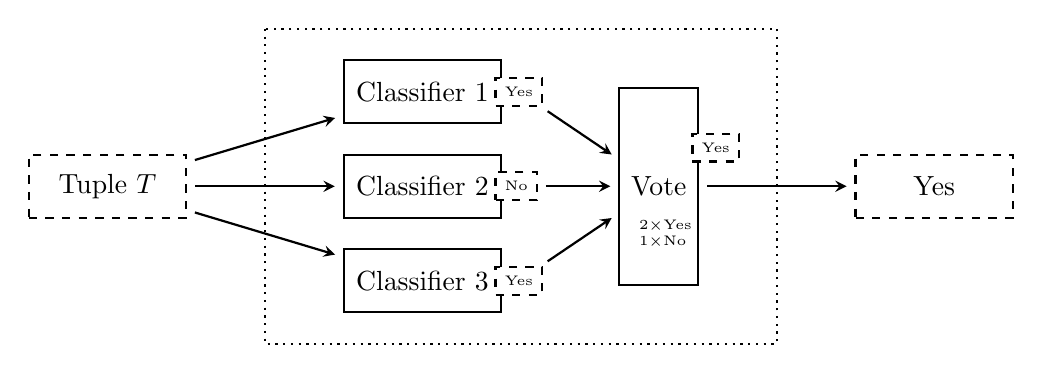
\begin{tikzpicture}
						\node[draw, thick, rectangle, minimum height=0.8cm, minimum width=2cm, dashed] at (0,0) (tuple) {Tuple $T$};

						\node[draw, thick, rectangle, minimum height=0.8cm, minimum width=2cm] at (4,1.2) (classifier1) {Classifier 1};
						\node[draw, thick, rectangle, minimum height=0.8cm, minimum width=2cm] at (4,0) (classifier2) {Classifier 2};
						\node[draw, thick, rectangle, minimum height=0.8cm, minimum width=2cm] at (4,-1.2) (classifier3) {Classifier 3};

						\draw[->, thick, shorten <=1mm, shorten >=1mm, >=stealth] (tuple) -- (classifier1);
						\draw[->, thick, shorten <=1mm, shorten >=1mm, >=stealth] (tuple) -- (classifier2);
						\draw[->, thick, shorten <=1mm, shorten >=1mm, >=stealth] (tuple) -- (classifier3);

						\node[right=-1mm of classifier1.east, draw, dashed, fill=white, thick] (classifier1decision) {\tiny Yes};
						\node[right=-1mm of classifier2.east, draw, dashed, fill=white, thick] (classifier2decision) {\tiny No};
						\node[right=-1mm of classifier3.east, draw, dashed, fill=white, thick] (classifier3decision) {\tiny Yes};

						\node[draw, thick, rectangle, minimum width=1cm, minimum height=2.5cm] at (7,0) (vote) {Vote};

						\draw[->, thick, shorten <=1mm, shorten >=1mm, >=stealth] (classifier1decision) -- (vote);
						\draw[->, thick, shorten <=1mm, shorten >=1mm, >=stealth] (classifier2decision) -- (vote);
						\draw[->, thick, shorten <=1mm, shorten >=1mm, >=stealth] (classifier3decision) -- (vote);

						\node[below=3mm of vote.center, text width=0.5cm, fill=white] (votecontent) {\tiny \centering 2$\times$Yes\\1$\times$No\\};

						\node[above right=3mm and -1mm of vote.east, draw, dashed, fill=white, thick] (votedecision) {\tiny Yes};

						\node[draw, thick, rectangle, minimum height=0.8cm, minimum width=2cm, dashed] at (10.5,0) (class) {Yes};

						\draw[->, thick, shorten <=1mm, shorten >=1mm, >=stealth] (vote) -- (class);

						\draw[thick, dotted] (2,2) rectangle (8.5,-2);
					\end{tikzpicture}
				}
			\end{center}

		\end{column}
	\end{columns}
\end{frame}

\begin{frame}{Bagging: Bootstrap Aggregation}
	\begin{itemize}
		\item \textbf{Analogy:}
		      \begin{itemize}
			      \item Diagnosis based on multiple doctors' majority vote.
		      \end{itemize}
		\item \textbf{Training:}
		      \begin{itemize}
			      \item Given a set $D$ of d tuples, at each iteration $i$, a training set $D_i$ of $d$ tuples is sampled with replacement from $D$ (i.e., bootstrap).
			      \item A classifier model $M_i$ is learned for each training set $D_i$.
		      \end{itemize}
		\item \textbf{Prediction in the case of classification: classify an unknown sample $X$.}
		      \begin{itemize}
			      \item Each classifier $M_i$ returns its class prediction.
			      \item The bagged classifier $M^*$ counts the votes and assigns the class with the most votes to $X$.
		      \end{itemize}
		\item \textbf{Prediction of a real number} (i. e. regression or time series forecast):
		      \begin{itemize}
			      \item Can be applied to the prediction of continuous values by taking the average value of each prediction for a given test tuple.
		      \end{itemize}
		\item \textbf{Accuracy:}
		      \begin{itemize}
			      \item Often significantly better than a single classifier derived from $D$.
			      \item For noisy data: not considerably worse, more robust.
			      \item Proved improved accuracy in prediction.
		      \end{itemize}
	\end{itemize}
\end{frame}


\begin{frame}{Boosting}
	\begin{itemize}
		\item \textbf{Analogy:}
		      \begin{itemize}
			      \item Consult several doctors, based on a combination of weighted diagnoses -- weight assigned based on the previous diagnosis accuracy
		      \end{itemize}
		\item \textbf{How boosting works:}
		      \begin{itemize}
			      \item Weights are assigned to each training tuple.
			      \item A series of $k$ classifiers is iteratively learned.
			      \item After a classifier $M_i$ is learned, the weights are updated to allow the subsequent classifier, $M_{i+1}$ to pay more attention to the training tuples that were misclassified by $M_i$.
			      \item The final $M^*$ combines the votes of each individual classifier, where the weight of each classifier's vote is a function of its accuracy.
		      \end{itemize}
		\item \textbf{Classification:}
		      \begin{itemize}
			      \item Each classifier $M_i$ returns its class prediction.
			      \item The bagged classifier $M^*$ counts the votes and assigns the class with the most votes to $X$.
		      \end{itemize}
		\item \textbf{Boosting algorithm can be extended for numeric prediction.}
	\end{itemize}
\end{frame}


\begin{frame}{AdaBoost ("Adaptive Boosting" \footfullcite[Algorithm AdaBoost.M1 on p. 131]{freund1997}): Training}
	\vspace*{-1em}
	\begin{itemize}
		\item \textbf{Given a data set $D$ of $d$ class-labeled tuples: $(x_1 , y_1), \ldots, (x_d, y_d)$} with $y_d \in Y = \{1, \dots, c\}$.
		\item \textbf{Initialize empty lists to hold information per classifier:} $\textbf{w}, \boldsymbol{\beta}, \textbf{M} \leftarrow $ empty list.
		\item \textbf{Initialize weights for first classifier to hold same probability for each tuple:} $w_j^1 \leftarrow \frac{1}{d}$
		\item \textbf{Generate $K$ classifiers in $K$ iterations. At iteration $k$,}
		      \begin{enumerate}
			      \item Calculate ``normalized'' weights: $\textbf{p}^k = \frac{\textbf{w}^k}{\sum_{j=1}^d w_j^i}$
			      \item Sample dataset with replacement according to $\textbf{p}^k$ to form training set $D_k$.
			      \item Derive classification model $M_k$ from $D_k$.
			      \item Calculate error $\varepsilon_k$ by using $D_k$ as a test set as follows: $\varepsilon_k = \sum_{j=1}^{d} p^k_j \cdot \text{err}(M_k, x_j, y_j)$,\\
			            where the \textit{misclassification error} $\text{err}(M_k, x_j, y_j)$ returns 1 if $M_k(x_j) \neq y_j$, otherwise it returns $0$.
			      \item If $\text{error}(M_k)>0.5$: Abandon this classifier and go back to step 1.
			      \item Calculate $\beta_k = \frac{\varepsilon_k}{1 - \varepsilon_k}$.
			      \item Update weights for the next iteration: $w^{k+1}_j=w^k_j \beta^{1-err(M_k, x_j, y_j)}_k$. \textit{If a tuple is misclassified, its weight remains the same, otherwise it is decreased.} Misclassified tuple weights are increased relatively.
			      \item Add $\textbf{w}^{k+1}$, $M_k$, and $\beta_k$ to their respective lists.
		      \end{enumerate}
	\end{itemize}
\end{frame}

\begin{frame}{AdaBoost ("Adaptive Boosting" \footfullcite[Algorithm AdaBoost.M1 on p. 131]{freund1997}): Prediction}
	\begin{itemize}
		\item \textbf{Initialize weight of each class to zero.}
		\item \textbf{For each classifier $i$ in $k$ classifiers:}
		      \begin{enumerate}
			      \item Calculate the weight of this classifier's vote: $w_i = \log(\frac{1}{\beta_i})$.
			      \item Get class prediction $c$ for (single) tuple $x$ from current weak classifier $M_i$: $c = M_i(x)$.
			      \item Add $w_i$ to weight for class $c$.
		      \end{enumerate}
		\item \textbf{Return predicted class with the largest weight.}
		\item Mathematically, this can be formulated as:
		      \begin{align*}
			      \textstyle M(x)= \arg \max_{y\in Y} \sum_{i=1}^k (\log \frac{1}{\beta_i})M_i(x)
		      \end{align*}
	\end{itemize}
\end{frame}

\begin{frame}{Random Forest\footfullcite{breiman2001}}
	\begin{itemize}
		\item Ensemble method consisting only of decision trees where each tree has been generated using random selection of attributes at each node.
		\item Classification: Each tree votes and the most popular class is returned.
		\item \textbf{Two methods to construct random forests:} (each builds $k$ trees)
		      \begin{enumerate}
			      \item \underline{Forest-RI} (random input selection):
			            \begin{itemize}
				            \item Random sampling with replacement to obtain training data from $D$.
				            \item Set $F$ as the number of attributes to determine split at each node. $F$ is smaller than the number of available attributes.
				            \item Construct decision tree $M_i$ by randomly select candidates at each node. Use CART to grow tree to maximum size without pruning.
			            \end{itemize}
			      \item \underline{Forest-RC}: Similar to Forest-RI but new attributes (features) are generated by linear combinations of existing attributes to reduce correlation between individual classifiers. At each node, attributes are randomly selected.

		      \end{enumerate}
		\item \textbf{Comparable in accuracy to AdaBoost, but more robust to errors and outliers.}
		\item \textbf{Insensitive to the number of attributes selected for consideration at each split, and faster than bagging or boosting.}
	\end{itemize}
\end{frame}

\begin{frame}{Classification of Class-imbalanced Data Sets}
	\vspace*{-0.5em}
	\begin{block}{Class-Imbalanced Data}
		\textit{Class-Imbalanced Data} refers to data where the main class of interest (positive labeled) is only represented by a small number of tuples. E.g., medical diagnosis and fraud detection.
	\end{block}
	\begin{itemize}
		\item Problem because traditional methods assume \textit{equality between
			      classes},\\ i. e. a balanced distribution of classes and equal error
		      costs.
		\item \textbf{Typical methods for imbalanced data in binary classification:}
		      \begin{enumerate}
			      \item \textbf{\color{airforceblue}Undersampling/Oversampling:} Changes distribution of tuples in training data.
			            \begin{itemize}
				            \item \textit{Undersampling:} Randomly eliminate tuples from negative class.
				            \item \textit{Oversampling:} Re-samples data from positive class.\\ For instance, method SMOTE generates synthetic data that is similar to existing data using nearest neighbor.
			            \end{itemize}
			      \item \textbf{\color{airforceblue}Threshold-moving:} Moves the decision threshold, $t$, so that the rare-class tuples are easier to classify, and hence, less chance of costly false-negative errors. Works when class returns a probability.
			      \item \textbf{\color{airforceblue}Ensemble techniques}.
		      \end{enumerate}
		      Threshold-moving and ensemble methods work well on extremely imbalanced data.
		\item \textbf{Still difficult on multi-class tasks.}
	\end{itemize}
\end{frame}

\section{Summary}

\begin{frame}{Summary}
	\begin{itemize}
		\item \textbf{Cluster analysis:}
		      \begin{itemize}
			      \item Groups objects based on their similarity and has wide
			            applications.
		      \end{itemize}
		\item \textbf{Measure of similarity:}
		      \begin{itemize}
			      \item Can be computed for various types of data.
		      \end{itemize}
		\item \textbf{Clustering algorithms can be categorized into:}
		      \begin{itemize}
			      \item Partitioning methods ($k$-means and $k$-medoids).
			      \item Hierarchical methods (BIRCH and CHAMELEON; probabilistic
			            hierarchical clustering).
			      \item Density-based methods (DBSCAN, OPTICS, and DENCLUE).
			      \item Grid-based methods (STING, CLIQUE).
			      \item Model-based methods.
		      \end{itemize}
		\item \textbf{Quality of clustering results.}
	\end{itemize}
\end{frame}

\begin{frame}[c]
	\begin{center}
		{\bf Any questions about this chapter?}\\[0.5cm]
		Ask them now or ask them later in our forum: \\\bigskip
		StudOn Forum \\
		\faLink\ \url{https://www.studon.fau.de/frm5045379.html} \smallskip

	\end{center}
\end{frame}

\section*{Appendix}

\section*{Appendix}

\begin{frame}{A Brief History of Data Mining Society}
	\begin{itemize}
		\item \textbf{1989 IJCAI Workshop on Knowledge Discovery in 
		Databases:}\\
		Knowledge Discovery in Databases (G. Piatetsky-Shapiro and W. Frawley, 
		1991).
		\item \textbf{1991-1994 Workshops on Knowledge Discovery in 
		Databases:}\\
		Advances in Knowledge Discovery and Data Mining (U. Fayyad, G. 
		Piatetsky-Shapiro, P. Smyth and R. Uthurusamy, 1996).
		\item \textbf{1995-1998 International Conferences on Knowledge 
		Discovery in Databases and Data Mining (KDD’95-98):}\\
		Journal of Data Mining and Knowledge Discovery (1997).
		\item \textbf{ACM SIGKDD conferences since 1998 and SIGKDD 
		Explorations.}\\
		\item \textbf{More conferences on data mining:}\\
		PAKDD (1997), PKDD (1997), SIAM-Data Mining (2001), (IEEE) ICDM (2001), 
		etc.
		\item \textbf{Journal ACM Transactions on KDD starting in 2007}.
	\end{itemize}
\end{frame}

\begin{frame}{Conferences and Journals on Data Mining (I)}
	\textbf{KDD Conferences:}
	\begin{itemize}
		\item ACM SIGKDD Int. Conf. on Knowledge Discovery in Databases and 
		Data Mining (KDD).
		\item SIAM Data Mining Conf. (SDM).
		\item (IEEE) Int. Conf. on Data Mining (ICDM).
		\item European Conf. on Machine Learning and Principles and Practices 
		of Knowledge Discovery and Data Mining (ECML-PKDD).
		\item Pacific-Asia Conf. on Knowledge Discovery and Data Mining (PAKDD).
		\item Int. Conf. on Web Search and Data Mining (WSDM).
	\end{itemize}
\end{frame}

\begin{frame}{Conferences and Journals on Data Mining (II)}
	\textbf{Other related conferences:}
	\begin{itemize}
		\item DB conferences: ACM SIGMOD, VLDB, ICDE, EDBT, ICDT, \ldots
		\item Web and IR conferences: WWW, SIGIR, WSDM, \ldots
		\item ML conferences: ICML, NIPS, ICLR \ldots
		\item PR conferences: CVPR, ICPR \ldots
	\end{itemize}
	\textbf{Journals:}
	\begin{itemize}
		\item Data Mining and Knowledge Discovery (DAMI or DMKD).
		\item IEEE Trans. On Knowledge and Data Eng. (TKDE).
		\item KDD Explorations.
		\item ACM Trans. on KDD.
	\end{itemize}
\end{frame}

\begin{frame}{Starting points to Find References? (I)}
	\textbf{Data mining and KDD (SIGKDD: CD-ROM):}
	\begin{itemize}
		\item Conferences: ACM-SIGKDD, IEEE-ICDM, SIAM-DM, PKDD, PAKDD, etc.
		\item Journal: Data Mining and Knowledge Discovery, KDD Explorations, 
		ACM TKDD.
		\item KDnuggets: \url{www.kdnuggets.com}.
	\end{itemize}
	\textbf{Database systems (SIGMOD: ACM SIGMOD Anthology CD-ROM):}
	\begin{itemize}
		\item Conferences: ACM-SIGMOD, ACM-PODS, VLDB, IEEE-ICDE, EDBT, ICDT, 
		DASFAA.
		\item Journals: IEEE-TKDE, ACM-TODS/TOIS, JIIS, J. ACM, VLDB J., Info. 
		Sys., etc.
	\end{itemize}
	\textbf{AI \& Machine Learning:}
	\begin{itemize}
		\item Conferences: Machine learning (ML), AAAI, IJCAI, COLT (Learning 
		Theory), CVPR, NIPS, etc.
		\item Journals: Machine Learning, Artificial Intelligence, Knowledge 
		and Information Systems, IEEE-PAMI, etc.
	\end{itemize}
\end{frame}

\begin{frame}{Starting points to Find References? (II)}
	\textbf{Web and IR:}
	\begin{itemize}
		\item Conferences: SIGIR, WWW, CIKM, etc.
		\item Journals: WWW: Internet and Web Information Systems.
	\end{itemize}
	\textbf{Statistics:}
	\begin{itemize}
		\item Conferences: Joint Stat. Meeting, etc.
		\item Journals: Annals of Statistics, etc.
	\end{itemize}
	\textbf{Visualization:}
	\begin{itemize}
		\item Conferences: CHI, ACM-SIGGraph, etc.
		\item Journals: IEEE Trans. Visualization and Computer Graphics, etc.
	\end{itemize}
\end{frame}

\end{document}
